\documentclass[a5paper]{article}

\usepackage{geometry}
\usepackage[utf8]{inputenc}
\usepackage{graphicx}
\usepackage[unicode]{hyperref}			%unicode pro nadpisy (labely)
\usepackage{tabularx}
\usepackage[english]{babel}
\usepackage{relsize}
\usepackage{sectsty}
\usepackage{longtable}					% kvuli seznamu ve slovniku pres dve stranky
\usepackage{ulem} 						% preskrtnuty text
\usepackage{lmodern}

\def\readyForPrint{0} % switch pro tisk [0:preview, 1:tisk]		%pro spravne nacitani fontu

\geometry{
	twoside,
	outer=7mm,
	inner=12mm,
	top=10mm,	
	bottom=15mm,
	footskip=8mm,
}
 
\sloppy

%\addtolength{\textwidth}{0.8in}
%\addtolength{\textwidth}{10pt}
%\addtolength{\textheight}{50pt}

\setlength\parindent{1.5em}
\setcounter{tocdepth}{2}

\if\readyForPrint1
	\usepackage[
		b5,
		cam,
		pdftex,
		center
	]{crop}	
\fi	

\allsectionsfont{\sffamily\mdseries\larger}
\subsubsectionfont{\it\sffamily\mdseries\larger}

%adresa budovy
\newcommand\budovaInfo[6]{
	\begin{center}
	\begin{tabularx}{0.9\textwidth}{ |l|X| }
		\hline
	    \textsf{Address} & #1 \\ \hline
	    \textsf{Residents} & #2 \\ \hline
	    \textsf{Tips} & #3 \\ \hline
	    \textsf{Lecture rooms} & #4 \\ \hline
		\textsf{Where to eat} & #5 \\ \hline
		\textsf{Bikes} & #6 \\ \hline
	\end{tabularx}
	\end{center}
	\noindent
}
\newcommand\budovaKratce[2]{
	\begin{center}
	\begin{tabularx}{0.9\textwidth}{ |l|X| }
		\hline
	    \textsf{Adress} & #1 \\ \hline
	    \textsf{Residents} & #2 \\ \hline
	\end{tabularx}
	\end{center}
	\noindent
}
%adresa budovy - zkracena
\newcommand\budovaAdresa[1]{
	\begin{center}
	\begin{tabularx}{0.9\textwidth}{ |l|X| }
		\hline
	    \textsf{Address} & #1 \\ \hline
	\end{tabularx}
	\end{center}
	\noindent
}

\newcommand{\subsubsubsection}[1]{
	\vspace{5pt}
	\noindent
	\textbf{#1}\\*
}

\newcommand{\nadpis}[1]{{
	\huge{
		\textsf{
			\centerline{
				\textbf{#1}
			}
			\vskip5
			\bigskipamount
		}
	}
}}

\newcommand{\uv}[1]{``#1"}

\def\ra{$\rightarrow$}


\begin{document}
\if\readyForPrint0
	\tableofcontents
\pagenumbering{gobble}
\vspace*{\fill}
\noindent This edition was completed thanks to David Nápravník, Miroslav
Štochel,
Anička Yaghobová, Vojtěch Švandelík, Klára Šarová, Meggy Calábková,
Kačka Žilavá, Martin Mach, Pavel Obdržálek
and many authors from the previous years whose texts still can be found here.
\\\\
Prepared for printing by David Nápravník, the cover designed by Filip Kreuziger,
translated by Anna Hotmarová.
\\\\
Many thanks for printing and publishing this edition belong to doc. Martin Vlach
and MatfyzPress.
\\\\
This edition's closing date was 10. 9. 2019, printed in 150 copies.
\\\\
The whole Cookbook is under the license \textit{Creative Commons State the
author -- Do not use for commercial purposes -- Preserve the 3.0 license}, where
the author is Matfyzák,
spolek studentů a přátel MFF UK.
\newpage
\pagenumbering{arabic}
\fi
\nadpis {The Cookbook of Matfyz}
\noindent Whether you are reading this on your laptop, your phone or you are holding the printed version of this not just ordinary Cookbook, welcome. Hopefully you will find it to be quite useful.


Unfortunately this Cookbook will not provide you with a lamb stew recipe because it is too complicated.
However, you will find here many recipes describing how to survive studying at Matfyz (which in Czech is short for ``the Faculty of Mathematics and Physics'').
Although we would like to let you discover the beauties of our faculty buildings, metro tunnels and Prague's numerous spires on your own, we believe that a little help might come in handy, at least in the beginning.
It might spare you a lot of embarrassing situations and misunderstandings and it will certainly make your transition to a new school less stressful.
This Cookbook was created as a student handbook giving details about the buildings of MFF (or MFF UK which in Czech stands for ``the Faculty of Mathematics and Physics at Charles University''), life in dormitories (mostly in the student residence 17. listopadu) and using the Prague public transport.


The first Student Cookbook was created in 1994 thanks to Martin Krynický (the 1998 version is available here).
From that time on new and new authors, members of Spolek Matfyzák (a group of the MFF's students organising various events and helping other students), try to improve the Cookbook by correcting old mistakes and subsequently adding new ones.
It is freely available online (\url{kucharka.matfyzak.cz}(CZ)) since 2011.


We will describe and explain almost everything here but some things are impossible to capture: the atmosphere of lectures, the presentations followed by applause or accompanied with laugh or loud snoring, the sleepless nights, the weeks and semesters spent writing the physics laboratory protocols, the first grades in SIS (Study Information System), the exams successfully passed talking over tea offered by a professor or even the failed exams.	
\section{Basic information about Matfyz}
The Faculty of Mathematics and Physics is one of seventeen faculties of the Charles University and it is, of course, by far the best one. 
It was established in 1952 when Vojtěch Jarník succeeded, using mathematical induction, in proving that Lenin evolved from monkeys and was expelled from the Faculty of Science at Charles University. Exasperated, he climbed the Albertov stairs, sat down on the grass and then wrote down all of his differential and integral calculus. 
The Dean's office was later built on this sacred place. 
Nowadays it is possible to find the faculty buildings in almost half of the city.
Almost 3000 students (including PhD students), of which approximately 500 are in their first year, are educated with the (sometimes even overly) enthusiastic help of more than 500 teachers with various degrees. Every fourth student is female. 
The students travel among four locations our faculty is based in (Karlín, Karlov, Malá Strana, Troja), Charles University Sports Center (SCUK) in Hostivař, dormitories and refectories.
Each of the buildings has its characteristic name, address and way of naming its lecture rooms which cannot be understood.
	\subsection{Study}
Studying at our faculty might seem challenging but if you follow the recommended
course of study, it might even become enjoyable.
All information about the obligatory courses, the recommended courses of study
and other duties can be found on the faculty's website.
A number of students unfortunately does not even make it through the first two
semesters of study but if you manage to overcome these difficult beginnings, you
will have a very good chance to successfully complete your studies.
Your older colleagues and teachers will give you a lot of useful advice but you
will not follow it and the night before an exam you will tell yourself: \uv{Why
did not I study more during the semester?}


\subsubsection{Study Programmes}

Our faculty offers bachelor’s, master’s and doctoral degree programmes, given in
either Czech or English. You usually start with the bachelor's programme and end
with completing the master's programme, however some of the students choose to
continue and study in doctoral degree programmes. This Cookbook will only
mention the bachelor's and master's degree programmes and exceptions for Erasmus
and exchange students.

\subsubsubsection{Bachelor's Programme}
If you are a regular student of the English programme, you might become a
bachelor of Computer Science.
The study usually takes three years and you have to pay for it. Studies are
concluded with a state final examination. Necessary conditions for taking the
State Final Exam include passing all obligatory courses, obtaining the required
number of credits for elective courses, reaching a total of at least 180 credits
and submitting a completed thesis (for the thesis defence). However, it is
possible to take the State Final Exam even without submitting the thesis and
complete it during the following year.
If you manage to pass, congratulations, you are a bachelor (Bc.).
If you are an Erasmus student, you might either study Computer Science or
Physics.

\subsubsubsection{Master's Programme}
If you are a regular student of the English programme, you might choose between
becoming the master of Computer Science or the master of Mathematics. The
studies usually take two years and if you manage to pass the State Final Exam
(the necessary conditions also include passing all obligatory courses, obtaining
the required number of credits for elective courses, submitting a completed
thesis and reaching a total of at least 120 credits), congratulations, you are a
master (Mgr.).


\subsubsection{Study Programmes}
There are three study programmes offered for the students of the English
programmes (this does not concern the Erasmus students) -- bachelor of Computer
Science, master of Computer Science and master of Mathematics. The Erasmus
students might also participate in the study programmes for future teachers and
Physics.


\subsubsection{Courses}
A wide range of courses is offered by the faculty, you can find them and their
descriptions in the SIS.

\subsubsubsection{ECTS Credits}
The ECTS credits are awarded at the end of the semester if you manage to pass
the course.
It is important to have enough credits because otherwise you might not be
allowed to continue to the next section of the study or you might not
successfully complete your Erasmus programme.
The number of credits you might obtain after mastering the course is given and
cannot be changed.
Some of the courses (differs according to the programmes) are obligatory (you
have to complete these before the state final examination), some of them are
elective (you have to complete the prescribed part of these courses before the
state final examination) and some of them are optional (all courses other than
the obligatory and elective that are offered at the university are considered as
Optional courses for the corresponding curriculum; it is up to you whether you
decide to take some of these courses).

You need to attain in total at least the minimum number of 45 ECTS credits to
enrol in the next year (so if you manage to attain over 90 credits in your first
year, you do not even have to do anything in the second year). However, the
normal number of credits required for the registration in the next year is 60
(corresponding to the sum of the credits in the recommended course of study).
The credits obtained for the completion of obligatory and elective courses must
prevail those obtained for the mastery of optional courses -- for the first
three years of the bachelor's programme the credits for optional courses are
counted up to the limit of 15 \% for the purpose of the Annual Evaluation of
Study.
The normal and minimum numbers of credits required for registration in the next
study section might be found in Rules of Study at the Faculty of Mathematics and
Physics and Code of Study and Examination of Charles University, both these
documents and other useful ones might be found on the faculty website.
\textbf{"The Annual Evaluation of study"} monitores the progress at the end of
each study section. If you are a bachelor student in the first year, you should
make the Annual Evaluation of study also after first study section (after first
semester), when you need to obtain at least 12 course credits.
And do not be mistaken -- you will have to complete your obligatory and elective
courses even though you otherwise might have enough credits to continue in your
study.
180 ECTS credits in total are required to complete the bachelor's programme (if
you study for more than 5 years, the number of credits rises due to the minimum
number of credits for every study section).

If you are an Erasmus or exchange student, you do not need to worry about the
aforementioned information. But attention, if you do not succeed in obtaining
the number of credits set by your home university, you might have to pay back
the Erasmus scholarship (or at least a part of it).

If you will not be sure about something, do not hesitate to contact SKAS or
Spolek Matfyzák, you can use e.g. this email address \url{sos@matfyzak.cz}.

\subsubsubsection{Prerequisites and others}
Course enrolment may be restricted by certain conditions (requisites), of which
the most common are the following: prerequisite (a prerequisite to Course X is a
course that must be successfully completed before you can enrol in Course X),
corequisite (a corequisite to Course X is a course that you have to enrol in at
the same time as Course X, or that you have already successfully completed) and
prohibited combination or incompatibility (courses X and Y are a prohibited
combination if it is impossible to enrol in Course X when you have already
completed, or you enrol in, Course Y).
In some cases, it is specified that completion of Course Y is equivalent, with
respect to the requirements of the curriculum, to completion of Course X; these
two courses are called equivalent or interchangeable.

If you are an Erasmus or exchange student, you do not have to worry about the
prerequisites and corequisites -- your Learning Agreement has been already
approved before your arrival to Prague based on your previous study results. And
sometimes it has not been easy to create a suitable Learning Agreement.

\subsubsubsection{Exams}
You have up to three attempts to pass an exam (provided there are still dates
available) but we strongly recommend preparing as well as you can for the first
attempt. If you do not succeed in passing the exam or obtaining the course
credit for a course, you are allowed to take the course again in the next
section of study, but a course can be repeated once at most. This information
however only applies to the regular students of the English programmes and not
to Erasmus students and exchange students.

There are four possible outcomes for an exam (the corresponding numerical values
and Czech equivalents are given in parentheses): Excellent (1 - Výborně), Very
good (2 - Velmi dobře), Good (3 - Dobře), Fail (4 - Nevyhověl). You pass an exam
if you obtain a grade of Excellent, Very good or Good; otherwise you fail.
The grades of Excellent and Very good have one advantage -- if you will need to
once again enrol at our university, you do not have to repeat these courses
(although that should not bother you in the best case).
How such an exam looks like? Exams are taken during the examination period at
the end of the semester and can be oral, written, or a combination of both
mentioned possibilities.
During the oral exam you usually have to choose a paper with the assignment,
then you have time to think and write down your solutions, and then talk about
it with the teacher. He might even let you to correct your mistakes. Sometimes
the exam takes even 8 hours.
If you are an Erasmus or exchange student, you will find the grade scale for the
conversion of your grades (so your courses could be successfully recognized at
your home university) at the back side of your official Transcript of Records
that you will get after completing all of your exams. It will also contain the
signature of the Vice-Dean for Students Affairs.

The examiners announce the exam dates via the SIS so it might be beneficial to
enable emails notifying you about the recently announced dates.
If none of the exam dates is convenient for you, you did not pass the exam at
the first attempt or you did not manage to pass it in time, do not be afraid to
contact the teacher and ask him to announce another exam date.
Most of the teachers are forthcoming and will allow you to try to pass your exam
e.g. at the end of July.

\subsubsubsection{Course credits and others}
Not every course has to be concluded with an exam, although most of the
obligatory ones are. To be even able to take an exam you usually need to obtain
a course credit.
A course credit (usually for classes) is awarded at the end of the semester. The
conditions for obtaining a course credit differ according to the course and
conditions defined by the teacher, for example involving the completion of a
test, programming an application, or writing a survey, and are specified by the
teacher at the beginning of the semester. The possible outcomes are Pass (in
Czech Započteno - Z) and Fail (Nezapočteno - K).
Erasmus students, pay attention to the courses that are not concluded with an
exam and agree with your home university in advance how such a course will be
recognized. Some of the partner universities award the gain of a course credit
(without a grade) with the worst grade possible.

\subsubsubsection{PE and languages}
It is great if you manage to learn at least a few Czech words or sentences that
will help you with the everyday communication during shopping, eating out or
travelling. And Czechs will be always pleased that you try to speak their
language.
Czech is not an easy language but the patient lecturers will help you to
familiarize yourself with at least the basics.
Apart from the Czech language you can also study e.g. German, Spanish or French
for free at Matfyz. Note to the Erasmus students: these courses are not awarded
with a grade, you will just obtain a course credit (and no grade).
And if these options are not sufficient for you, you can study for example
Korean, Portuguese or Russian at the Faculty of Arts at Charles University. Also
for free.

Concerning the physical education, Matfyz offers a wide range of PE classes
(from swimming and soccer to canoeing). It is said that the traditional sport of
Matfyz is volleyball -- there are regularly organized tournaments for for both
-- students and professors.

\subsubsection{Recommended course of study}
You do not need to follow any set course of study if you do not want to. To
enrol into the next section of study you just have to obtain enough ECTS credits
(in the right ratio of the credits attained for the completion of obligatory,
elective and optional courses) and complete all of the obligatory courses till
the end of your studies.
However, sometimes it is difficult to make sense of all of the prerequisites and
corequisites so the faculty has prepared the recommended course of study to help
you with that.
The recommended course of study is not binding, however it is advisable to
follow it. If you do so, you should be able to fulfil the requisites (see below)
considering the relations between the courses. It is also the best way to
achieve the timely graduation.
Every degree programme has its recommended course of study and you will find it
either in the SIS, in the Study guide or on the website. This information only
applies to the regular students of the English programme.

It is probably best to follow the recommended course of study, at least in the
first year. You might even enrol in some optional courses from the higher years
that you do not need to successfully complete (there are no sanctions for not
completing the optional courses, except for the possibility of not gaining the
scholarship).


\subsubsection{Student Affairs Department}
Your student advisors deal with all of your applications and issues -- the
joyful ones (such as successfully completing your studies) as well as the sad
ones (such as the exclusion).
%The students of each programme have one officer that takes care of all their
problems, the first year students have their own officers (so please be nice to
her).
The student advisors are also Erasmus coordinators for incoming students and
they take care of the other exchange students as well. Please bear this in your
mind when requesting information which can be easily found on the faculty
website.

Usually you will not encounter any queues at this department, with the exception
of some important deadlines. If you ever wanted to complain about the Student
Affairs Department, remember that Student Affairs Department at Matfyz is one of
the most pleasant compared to the other faculties.


\subsubsection{SIS}
The Study Information System (SIS) is most of the times a functional system that
decreases the need of the student and the Student Affairs Department
communicating in person.
The whole university uses it so if you are angry with it, just think about how
difficult it must be for the students of philosophy to deal with it and you
should immediately feel better. The link is \url{is.cuni.cz/studium/eng/}.

The SIS accompanies you during your whole studies. You have probably encountered
it when you submitted your study application.
You will also use it to enrol in courses, look up your timetable or while
ignoring the fact that some of your courses overlap (the obligatory courses
never overlap if you follow the recommended course of study, however it is not
possible to prevent the overlapping of optional courses).

You will also use it to sign up for the exams and then check your results. You
can also find there following information: about teachers, classes and their
locations and their language of instruction etc.


\subsubsection{Scholarships}
You might obtain a scholarship for outstanding academic achievement. Another
types of scholarships are different types of grants and the scholarship for RDI
(Research, Development, and Innovation) activities in accordance with special
legislation.
It is recommended to put your bank account number to the SIS at the beginning of
your study so the scholarships might be easily paid to you. The opportunity for
getting these scholarships applies only to the regular students of the English
programme.

\subsubsubsection{Scholarship for outstanding academic achievement}
The scholarship for outstanding achievement is awarded at the end of the
academic year; in the first year it is awarded also for the first study section
which means based on the exam results from the winter semester -- if you will
study hard from the start, you might get an allowance for the holidays.
The Dean decides how high this scholarship will be each year and it is awarded
according to two criteria -- the year and the average result of study (it also
contains the results of exams which you failed on your first try).
Attaining at least the normal number of credits is one of the necessary
conditions for obtaining a scholarship for excellent study achievement but
usually it is awarded to students who obtained at least 60 ECTS credits (30 in
the first study section), their actual period of current study has not exceeded
the standard period of study (3 years for the bachelor's programme) and their
weighted average grade achieved has not exceeded the set limit.
The detailed rules for awarding the scholarship can be found in Rules for
Awarding Scholarships and Bursaries at the Faculty of Mathematics and Physics.

\subsubsubsection{Scholarship for Outstanding RDI (Research, Development, and
Innovation), Artistic, or Other Creative Achievement Contributing to Greater
Knowledge
(\uv{the Scholarship for Outstanding Achievement})}
The scholarship for outstanding achievement
The Scholarship for Outstanding Achievement may be awarded, in compliance with
the conditions set out in the Rules, to students who have achieved, or
participated in the achievement of, an outstanding scientific result. An
outstanding scientific result means in particular publication of a research
paper or giving a presentation at a scientific conference.

\subsubsubsection{Grants}
Finally we will mention the special form of bursaries in cases worthy of special
consideration. It is a bursary for student projects funded from Faculty Student
Grants (\uv{the FSG}); the Dean decides on the awarding thereof twice a year,
once in autumn and once in spring.
Any student or group of students of full-time bachelor’s or master’s programme
of study at the Faculty can apply for the FSG bursary. An applicant may file no
more than one proposal for the FSG bursary in a given period (autumn or spring);
the same applies even if the student is a member of a group of applicants.

\subsubsubsection{Scholarship for RDI (Research, Development, and Innovation)
Activities in Accordance with Special Legislation and Doctoral bursary}
While studying in the master's programme and the doctoral study, you will have
more options to get the scholarships -- various scholarships for RDI activities
in accordance with special legislation or even state grants (for details write
to the Research and International Affairs Department
(\url{mensikova@dekanat.mff.cuni.cz}) or visit the officers personally, room
next to the office of your Student Advisor -- as the website about research and
grant activities is available only in Czech in this moment)\dots and of course,
the PhD students get their \uv{salary} in the form of doctoral bursary.	
	\subsection{Faculty buildings}
The Faculty of Mathematics and Physics is based at several locations in Prague.
Most often you will visit one of these four locations: Karlov (where the Dean's
departments can be found and the students of Physics have most of their lectures
there), Malá Strana (where most of the students of Computer Science have their
lectures), Karlín (the students of Mathematics usually have their lectures
there) and Troja (there are labs and lecture rooms of the students of Physics
and there are also lecture rooms used for the purposes of language education).


\subsubsection{Karlov}
Two neighbouring faculty buildings are based there, in the street Ke Karlovu.

\budovaInfo{Ke Karlovu 3, Prague 2}
{Mathematicians, physicists}
{It houses the Dean's departments and Student Affairs Department and you can get
your ISIC card sorted out in the basement.
M1 is our largest lecture room and physics practical classes take place there.}
{Names of the rooms start with the letter \uv{M} (M1, M2, M3, M5 a M6).}
{The refectories Albertov and Budeč are the closest ones. You might use the jug
kettle or microwave located in the lab.}
{Bike-stands are in the courtyard.}

\budovaInfo{Ke Karlovu 5, Prague 2}
{Physicists}
{It houses the Institute of Physics of Charles University and you can find the
Foucault pendulum there.}
{Names of the rooms start with the letter \uv{F} (F1, F2 a KFK)}
{The closest refectories are Albertov and Budeč. You might use the jug kettle or
microwave located in the lab of the building M.}
{Bike-stands are in the courtyard of the building M.}

\subsubsection{Malá Strana}

\budovaInfo{Malostranské náměstí 25, Prague 1}
{Computer scientists}
{The oldest and most beautiful faculty building. There is an 11th century
rotunda of St. Wenceslas and also Rotunda, the most important lab for the
students of computer science. The building is almost always locked because of
tourists, you need an ISIC card to enter.}
{Names of the rooms start with S \uv{S} (S1, S3, \dots, S11), four IT classrooms
(SW1,
SW2, SU1, SU2), Rotunda, lots of other lecture rooms. The whole building is
often called MS (short for Malá Strana).}
{The restaurant Profesní dům with student discounts is located in the basement
of this building. Other options include McDonald's, Biomarket Vacek and a
chinese restaurant near Karlův most. If you follow the tramway for about 100 m
in the direction of Újezd (not through the tunnel), you will come across another
chinese restaurant and Subway.
The closest refectory is located in the building of the Faculty of Law -- take
the tram no. 15 or just walk across Mánesův most. There is also a school canteen
in Dražického náměstí.
A microwave is located on the 4th floor of this building (in front of S1) at the
end of the left corridor.
}
{Bike-stands are in the left corridor (in front of SW2) and in the courtyard.}


\subsubsection{Karlín}

\budovaInfo{Sokolovská 83, Prague 8}
{Mathematicians}
{The best room of MFF is situated in the basement --\textit{Respirium} and it
has a jug kettle, microwave and a place to relax. The shop of MatfyzPress is
based on the ground floor.}
{\uv{K} (K1--K12) + other lecture rooms.}
{The refectory Jednota is just a few stops by tram away. There are also lots of
fast food restaurant near the metro station and the shops Billa and Lidl are
also based in the street.}
{A stand in the courtyard (ring the bell for the reception).}

\subsubsection{Troja}
There is a whole building complex in Troja -- one high rise building, four low
rise buildings and one is being constructed. The main building is marked by T,
the high rise building by A, the building of the heavy technology laboratories
by L, the building of the research and development workrooms by V and the last
one is the cryogenics laboratory with the letter C.
The building housing the IT classrooms is still being constructed and the works
should be finished at the end of 2019.
You can find a map of this complex at the end of the Cookbook.

\budovaInfo{V Holešovičkách 2, 180 00 Prague 8}
{Physicists}
{The Faculty of Nuclear Sciences
and Physical Engineering of the Czech Technical University in Prague is also
based there, then you can find \textit{Van der Graff Generator} and the nuclear
sciences' reactor VR1 (code name \textit{Vrabec} -- Sparrow in English) in the
building L. The whole complex (with the exception of the building C) is
interconnected by the underground corridors.}
{Names of the rooms start with the letters \uv{T}, \uv{A}, \uv{V}, \uv{C} a
\uv{L} (T1, T2, T5--T10,
VxxxJAZ) + other lecture rooms located in the departments}
{There is a buffet in the building T, other options include shops and
restaurants near Nádraží Holešovice or Bulovka. }
{There are stands in front of all buildings in this campus. You can also leave
your bike in the entrance hall of the building C, opposite the porter's lodge.}
	\subsection{Buildings not beloning to the faculty}
The faculty buildings are not the only ones you will visit during your study. The most important of them is probably the Charles University Sports Center where most of the PE classes take place. 
Another buildings worth mentioning are Karolinum -- historical seat of the university that you will visit during the matriculation -- or the boathouse in Malá Chuchle where the canoeing classes take place.


\subsubsection{SCUK (Charles University Sports Center) Hostivař}
\budovaKratce{Bruslařská 10, 102 00 Prague 10 - Hostivař}
{PE teachers}
Its first floor houses the departments of physical education of some faculties, ours is located in the back.

You can find most of the changing rooms if you enter the building, go down the stairs and turn left (women's changing rooms are on the right, men's on the left). 
If you want to go to the swimming pool, borrow a padlock from a lady in the window facing the stairs and go to the changing rooms right next to this window. 
You need to have your own padlock for locking your locker in the other changing rooms.

The location of this building might become a reason you will hate PE because it is on the other side of Prague than all other faculty buildings.


\subsubsection{Karolinum (Charles University Rector's Office)}
\budovaKratce{Ovocný trh 5, 116 36 Prague 1}
{Bureaucrats}
Needles to say, the rector's office does not belong to the faculty. It is similar to our Dean's office but influences the whole university.
Two events usually take place in the famous ancient \textit{Karolinum}: \textit{matriculation} (anyone can experience one) and \textit{graduation} (just for those who made it through).


\subsubsection{Boathouse Malá Chuchle}
\budovaKratce{Strakonická Prague 5 - Malá Chuchle}
{PE teachers}
If you choose to visit canoeing classes, you will commute to Malá Chuchle in the first month of the winter semester and the last month(s) of the summer semester. You will squeeze in the swimming pool in Hostivař with the swimmers during the winter.
	\subsection{Labs}
The computer laboratories are called \textit{labs} for short. There is at least one in every faculty building, They are generally accessible by the students of Matfyz but there are also some computers belonging to the departments which only some of the students might use.

If you want to access the lab, you will need Charles University student card and a user account or an access to the SIS (Study Information System).
If you need to set up the account, you can apply for it in one of the labs and the account is established right away.
Every student of the Charles University might access the computers in Troja and Karlov. You log in with the same user name and password as if you tried to log in to SIS. 
Sometimes it is necessary to find the lab's administrator and undergo a training about the lab's specifics.

The labs may or might not be occupied depending on the time of the day, part of the semester and also the lab's location. Most people use the labs during the winter semester.
On the other hand, the lab in Karlov is usually empty because it is not easy to find it. Do not forget to follow the Dean's directive no. 4/2008 stating that you have to treat the computers well and that you cannot use illegal software or write abusive emails.

Every lab has a printer, the black and white printing costs 1 CZK for one A4, the colour printing from 5 to 15 CZK. Not all of the printers are able to print in colour.
Most of the labs also have a scanner.

Each of the labs has its own website, you can find the list here  \url{www.mff.cuni.cz/cs/vnitrni-zalezitosti/it-a-sluzby/pocitacove-laboratore}(CZ).

For more information about the labs check out the electronic version of the Cookbook:
 \url{www.matfyzak.cz/kucharka/index.php?title=Laby}(CZ).



\subsubsection{Alternatives}
It often happens that the computer lab is closed and your roommate needs the room to spend some joyful time with his girlfriend and sometimes it collides with the times you actually need to work.
If you have your own laptop, you can use the night study room in the National Library of Technology in Dejvice. It is opened any time, even when the library itself is closed, and there is wifi, electricity, toilets and vending machines.
However, you will need to make the registration some time during the day -- it costs 100 CZK per year.
	\subsection{Spolek Matfyzák}

The \textit{Spolek Matfyzák} is a group of the MFF’s students organising various events and helping other students -- its members are also the authors of this Cookbook. Any (even former) student of MFF or a person associated with Matfyz in any other way might become its member.

Its leader is called \textit{Náčelník} (``Chief") and he is surrounded by his \textit{Náčelnictvo}. There is also \textit{Rada starších} (``Council of Elders") that makes sure that everything happens according to the rules.
The website is \url{matfyzak.cz}(CZ) and you can reach them at spolek@matfyzak.cz or via Facebook.

Anyone can become a member, the members often change as students come and go.
\textit{Become an active member of Spolek Matfyzák!} If you like to organize various events, have inspiring ideas or you just want to chat with older students, this is the place to go. Just contact us. You will most definitely gain a lot of useful skills and make new friends.


\subsubsection{Beánie}
The \textit{Beánie} is a party held at the beginning of the semester.
The first year students become the ``proper students of Matfyz" during the ancient ``Jarníkův rituál" (``Jarník's ritual"). 
You can watch the cult movie Matfyzák and other movies created by the students of Matfyz, listen to the concerts of various bands and there are always some entertaining competitions and theatre plays. There is also the famous exhibition \textit{Matfyzák včera, dnes a zítra} (``the student of Matfyz yesterday, today and tomorrow") and you might buy some T-shirts with the logo of Matfyz and other items.
This event is meant mostly for the Czech students, but not exclusively and you are very much welcome to come. However, it is all in Czech so we recommend you to come with someone who can translate it for you.


\subsubsection{Matfyz Ball}
\textit{The Matfyz Ball} takes place in the beautiful Žofín ballroom. Every student tries to score some points with the teachers by showing his perfect dancing skills (because the examination period is coming and you never know what might be of use to you) or at least win some of the tombola prizes. 
You can buy the tickets a few weeks before the ball takes place in the library, at the dormitory or online. Book your tickets in advance as they usually sell out quickly.


\subsubsection{Other activities}
Besides these events we also organize a few others every year. Some of them take place at the student residence 17. listopadu -- e.g. \textit{KolejCup} (trivia quiz including lots of running) and \textit{Běh do schodů} (``Up the Stairs Run", it is probably clear what happens there, the all-time high is 1 min 36 sec).
Tour de Pub is another popular event -- more or less regular meetings in the pub where we drink beer or others drinks and just chat.
Spolek also tries to do some socially beneficial acts -- e.g. the members go donate blood together. Just regularly check our website or the notice boards at the faculty buildings and you will find out all the necessary information about the upcoming events.

Spolek also cooperates with other organizations, theatres (check our website for the discounts), sells T-shirts with the logo of Matfyz and other items (e-shop can also be found on our website) and manages this Cookbook.

\subsubsubsection{Activities of the university}
Apart from the MFF's events Spolek Matfyzák also participates in the events organized for all students of the Charles University, such as Studentský jarmark (``Student fair"). You can learn information about all of the things you can do while studying at the university, listen to the music, taste some great food and drinks and learn about other societies at the university.

Spolek Matfyzák also publishes invitations for other interesting university activities or lectures.


\subsubsection{Other societies and associations}
There are lots of other societies and associations at the university.There is also the Charles University Student Union (SU UK, \url{cssauk.cz}(CZ)) acts as a guide for university student organizations, facilitating communication and cooperation among them, developing a creative platform for active students, supporting the implementation of their ideas, and acting as a mediator providing information to all students about what is currently happening in the academic community.
Current events organized for the whole university are Studentský jarmark or Studentský majáles (``Student fair") and the CU Student Union also organizes discussions with famous people.
	\subsection[SKAS]{SKAS (Student Chamber of the Academic Senate)}
It represents students and their interests in self-governance of the faculty.
It has 9 members elected at the end of the academic year by \textit{you,
students}. Three representatives are elected each year for a three-year term.
The duties of the SKAS include controlling the way the faculty is run (more than
one third of the votes in the Academic Senate is theirs) and presenting the view
of the students to the Senate and the dean.
Therefore, do not forget to vote!

You can always turn to the SKAS, especially if you have any difficulties with
your study (e.g. the teacher takes a lot of time to correct the tests etc.) or
if you need any information about the study and do not know who else to ask.
\textbf{Remember that most of the problems can be solved, you just have to start
solving them as soon as possible.}

The contacts and other information about the activities and organization of the
SKAS can be found on the notice board in every building or on the website
\url{skas.mff.cuni.cz}(CZ).

\subsubsection{Student evaluation}
The student evaluation is supposed to enable the students to evaluate the
performance of their teachers.
You should complete it as it will help the other students and sometimes even the
teachers. They usually do not intend to make faults.
Please write comments (either positive or negative). Your teachers as
well as the faculty management will certainly read them and sometimes also
react.

The evaluation always happens during the examination period. It has taken
different forms during the last years, currently you will fill out your
evaluation online in the SIS where you can also find the results of the previous
evaluations.
	\subsection{ISIC}
Every student of the Charles University has to have a Charles University ID
card, usually called the ISIC (although you do not have to buy the ISIC
license).
It is a plastic card that you get during the enrolment. It might be used to
access some buildings, you might pay with it in the refectories and it is also a
proof that you are a student of Matfyz.
You also need to have a valid coupon for each academic year -- it is just a
little piece of paper but its absence renders the card invalid. You will always
get it during the enrolment.

You can also buy the ISIC license which means that you can use various discounts
offered by the ISIC company. It is usually valid till the end of the year (but
if you issue it in September or later, it will be valid to the end of December
of the following year) and you have to pay for it. The price is 230 CZK a year.
If you need to revalidate your ISIC card, just visit (after completing the paper
registration in the next study year) any of the ISIC office of the Charles
University. One of them is located in the basement of the building Ke Karlovu 3.
\section{Dormitories and refectories}
You will probably also want to stay and eat somewhere while studying in Prague. Most of the students stays at the student residence 17. listopadu, at least for a few years. 
Therefore most of this chapter will focus on it but it does not matter that you could not choose to stay anywhere else, lots of the students of Matfyz also stay at the other dormitories or in a flat.
	\subsection{Student residence 17.~listopadu}

The whole building complex of the student residence and refectory 17. listopadu
contains two dormitory buildings (buildings A and B) and the building of a
former refectory (building C, nowadays in possession of the Faculty of
Humanities and it is being reconstructed).
There are two basement floors under these buildings and you can find there the
refectory, technical support, bed linen deposit, gym, music rehearsal room and
lots of other more or less used space.

The basement of the buildings A and B is connected, although it is not easy to
find the way in the beginning.

\subsubsection{Building A}
The building A is the higher one (20 floors + ground floor) and is also closer
to the road. There are four lifts (but frequently just three of them are working
and sometimes, usually when you need it the most, even less) and two emergency
staircases.
There is an unwritten rule that says that you should not use a lift if you do
not need to go to the fourth floor and below, to go just one floor up
or down or to take it from the fifth and below floors to get to the
ground floor. You also should go to the -1 floor only during the lunch hours.
All of these trips are much faster if you use the stairs and it will save you
from the hateful stares of other passengers that usually go to the double-digit
floors.
But of course, the exceptions are allowed in the case of injury, exhaustion etc.

The windows either face the east (with a picturesque view of Magistrála) or the
west (with a view of the building C and tunel Blanka and the traffic jams
occurring there).
The east side is more popular with the residents as it is much cooler during the
summer.

The residents of the building A's twentieth floor about twice a year organize
parties in the corridors (although usually without permission of the
authorities). Do not rather move there if there is a chance this would bother
you.

There is a computer laboratory (\uv{lab}) on the ground floor. You will find
more information about it in the chapter about labs.
The offices are also located behind the lifts.


\subsubsection{Building B}
The building B has 16 floors + ground floor.

There is a dormitory council's room, piano room, gym and music rehearsal room in
the basement. On the ground floor you can find a study room, small shop for the
dormitory residents, ecumenical room and the office of the dormitory chief.

There are two small lifts and one emergency lift. It very often happens that at
least one of them does not go to all floors (especially the 15th floor) or does
not work at all. There is also an emergency staircase.
While you can frequently see a sign with \uv{MIMO PROVOZ} (out of order) on the
lifts in the building A, the lifts in the building B usually have the sign
\uv{VÝTAH V PROVOZU} (the lift is working). It is up to you to figure out the
hidden meaning of this.

The windows either face the east with the view of Milada (a former villa,
nowadays in ruins, and former squat that should have been demolished a long time
ago) or the west with the view of a hill.
Both of the sides of the building are hidden from the sun as the building A is
higher and offers shade.

\subsubsection{Former refectory (building C)}
Nowadays it is under construction. The Faculty of Humanities should move here
once the building is reconstructed because this faculty does not have its own
building.
Because all these buildings are interconnected, even the students that do not
have rooms close to the construction site are often disturbed by the noise.


\subsubsection{Magistrála}
Magistrála leads from Jižní Město to Prosek. It is a real blessing for our
dormitory as it makes a lot of noise and is like a poison for our lungs. Its
uses are endless.
Watching the road maintenance workers trying to get rid off the snow is a
distraction during the winter. Counting the passing cars can distract you while
studying for the exams. Plus it emits a nice low frequency sound helping you to
fall asleep.
Its illumination resembles the Greek letter epsilon.

A crowd of drivers, moving at the speed of a slow pedestrian, forms at
Magistrála every morning.
This might be beneficial for some people's confidence as they are easily able to
get ahead of the unnerved drivers.

After endless years of construction the tunnel complex Blanka has been connected
to Magistrála. In the afternoon there are usually traffic jams outside of it.


\subsubsection{Technical specialities}

Some people claim that if a fixed overcritical number of windows, all of them
above each other, is opened, the dormitory building falls down. It has not been
experimentally verified yet.
The building itself has the qualities of a chimney. While there used to be cold
on the lowest floors, you never needed to turn on your heating on the eighteenth
floor even if the weather was freezing, despite the fact that the building was
not thermally insulated at the time (residents staying on the highest floor used
to have different problems of course -- if you turned your heating on, you were
often unable to turn it off again).

The meteorologists will certainly gladly tell you why the wind is always strong
in the vicinity of the dormitory.
While there is just a gentle breeze blowing in Prague, the students walking
around the building A have problems to stay on their feet as the wind is very
strong. Only the luckiest ones manage to take a small step forward.
The whole trip along the (shorter!) wall of the building A might take a few
minutes. After a few windy days even the most stubborn student understands why
it is not always good to open the windows without checking whether you will not
need another three people to help you close them afterwards.

The construction works in the vicinity of the dormitory generally start at the
beginning of the examination period; it is hard to say whether this is just a
coincidence or an evil plan.
For example the anti-flood measures were built in the winter of 2009, the
reconstruction of the entrance hall took place in the summer of 2009, the
foundations of a building near the dormitory were laid in the summer of 2014,
the same went for the construction of the tunnel complex Blanka or the
reconstruction of the building C.


\subsubsection{Eduroam}
It is much easier to connect to Eduroam (university wifi network) now. You can
set you eduroam password in the CAS system. After this everything tends to work
the same way as if you tried to connect to any other wifi.
ATTENTION! your login name is: name@cuni.cz or isicnumber@cuni.cz.


\subsubsection{Dormitory council}
It is elected by the dormitory residents and represents their interests on the
regular meetings with the dormitory management.
You will find many useful information on their website -- important phone
numbers, forms, rules, lift etiquette, opening hours and a simulator for
organizing furniture.
Website address: \url{listopad.koleje.cuni.cz/lang/en}.

\subsubsection{Visits}
If your relatives or girlfriend/boyfriend are supposed to visit and you want to
accommodate them in your room, it is possible. You basically need to fulfil only
2 conditions. 1) Ask your roommate, if (s)he agrees and allows it and 2)
announce it in the accommodation office and at the reception -- or just at the
reception. The visitor will pay only 50 CZK per night.
Anyway, do not forget to keep the night silence (between 10 p.m. and 7 a.m.)
also during his/her visit.
	\subsection{Other Dormitories}
\budovaAdresa{
    The student residence Na Větrníku, Na Větrníku 1932, 162 00 Prague 6
    The student residence Kajetánka, Radimova 12, 169 00 Prague 6
}
While the student residence 17. listopadu has nice rooms but unpleasant surroundings, the student residence \textit{Na
Větrníku} (also called Větrák) has it the other way around -- there are nice surroundings and a park near the dormitory bud the rooms are small and ugly. On the other hand, it is very cheap.
The student residence \textit{Kajetánka} (also called Kajka) is located about 20 minutes away from Na Větrníku. Many students of medicine and computer science stay there.

\budovaAdresa{The student residence Areál Hostivař, Weilova 2, 100 00 Prague 10}
This dormitory is meant to accommodate the students of Erasmus or Erasmus+. There are single and double rooms (the price differs). The double rooms have its own toilets and there are also toilets on each floor. Some of the rooms but do not have its own toilets (the price also differs).
There is always one kitchen on each floor. It is a good place for meeting new people.
There is a study room, copy machine, coffee and tea vending machine and also a normal vending machine in the entrance hall. It is also possible to buy sandwiches at the reception.
The laundry room is located in the basement of the building 1.
There is a hairdresser and pizzeria in the complex of the dormitory buildings (on the terrace of the building A) and you can also find Charles University Sports Center in the vicinity, with a swimming pool, tennis courts and indoor hall.
The residents of the dormitory can connect to the university wifi network called eduroam. Your login name is: name@cuni.cz or isicnumber@cuni.cz. You should be able to set your password in the CAS system.

\budovaAdresa{
    The students residence Vltava, Chemická 953, 148 28 Prague 4 - Jižní Město
    The student residenc Otava, Chemická 954, 148 28 Prague 4 - Jižní Město
}
Someone says that these dormitories are good value for money, someone says that they are a bit far away from the city center. 
Lots of students of VŠE (University of Economics) stay here.

\budovaAdresa{The student residence Budeč, Wenzigova 20, 120 00 Prague 2}
The student residence \textit{Budeč} is located fairly close to Karlov. It is a small dormitory in the city center (7 min walk from I. P. Pavlova) and has about 225 residents who mostly know each other and organize small parties (and even big ones, about four times a year).
The rooms are a bit smaller and not all of them are the same size, some double rooms are as big as the rooms for three. 
The first three floors were reconstructed in 2017. The only disadvantage of this dormitory might be that all of the residents of one floor have a collective kitchen, two collective toilets and showers. Warning: the toilets and showers for men and women are not separated.
However, they are cleaned daily so do not worry about that.
One big advantage of this dormitory is its refectory, one of the best of the Charles University refectories.
Every floor has its own study room where you often find the students of medicine, law and philosophy. 
How can you get to MFF? Albertov is a 6 min walk. If you take the tram no. 22 from the I. P. Pavlova, you can get to Malostranské náměstí in $\pm$ 17 min (or in 14 min if you are in a hurry and use the metro). It takes about 20 min by the metro and bus to get to Trója.
Generally speaking, if you want to go anywhere, just set out half an hour earlier and you should get there in time.
Unfortunately, Hostivař is a bit far away even from this place. Just take the tram no. 22 from I. P. Pavlova or go two stops by metro to Hlavní nádraží and then go by train (runs once every half an hour). 
But the safest way is to take a book with you, get on the tram no. 22 and not hurry anywhere.

\budovaAdresa{The student residence Švehlova, Slavíkova 22, 130 00 Prague 3}
\textit{The student residence Švehlova} (also called Švehlovka) is also located in a nice historical building but it is larger then Budeč and has a theatre instead of a refectory.
It is situated near náměstí Jiřího z Poděbrad so it is not very close to any of the MFF's building but at the same time it is not that far away (including Hostivař!).


The Charles University has eleven dormitories in total just in Prague. All of them have different facilities and rooms, from single rooms to rooms for five people.
We will not mention all of them because we actually do not know much about some of them but we still believe that staying at the dormitory is a valuable experience and a part of the student's life and you should not miss it.
	\subsection{Important Refectories}
The refectories are the canteens of the Charles University. The food is paid for
with an ISIC card so you have to charge it in one of the refectories. You also
need to register yourself on your first visit (but this registration is then
valid for all of the Charles University refectories).
Your account will be set up and it will then enable you to pay or order meals
online (at least a day in advance). If you do not order your meals, you will
have to take anything that is left.

The price is about 50--80 CZK for students. You can usually choose from 4 meals
(at least one of them is vegetarian) and soup (single price 9.20 CZK), sometimes
you can also choose from more expensive (but luxury) meals.
The refectories are closed on weekends. Another way to feed yourself is to buy
subsidized sandwiches (for budget-friendly prices) at the dormitory receptions,
refectories and in some faculty buildings.


\subsubsection{Refectory Troja}
It is temporarily closed at the moment and it is not sure when it will reopen.
It has been substituted by a vending machine on the ground floor of the building
A but it is not really a sufficient replacement.

Once the refectory is opened, you will find it in the basement of the building A
(go down the stairs from the reception and turn left).


\subsubsection{Albertov (Albertov 7)}
It is located near the buildings in Karlov so it is very convenient for the
students of Mathematics (in their first year) and Physics. Althought the queues
are long, they tend to move quickly and you will most likely have no problem
with finding a place to sit.

The easiest way to get there from both of the faculty buildings in Karlov is to
take the path between these buildings and go straight ahead until you see a
building with a sign Menza on your right side.


\subsubsection{Budeč (Wenzigova 20)}
Another refectory in Karlov. It is noticeably smaller than the one in Albertov
so you might have some problems with finding a place to sit but they cook better
and the building was recently reconstructed.

The fastest way to get there from both of the faculty buildings is to go in the
direction of Nuselský most (which means turn right and then take left at the end
of the street), go through the pedestrian underpass, turn left and then right at
the nearest crossroads.
Another way how to get there from the faculty building is to turn left and then
right at the crossroads with Wenzigova street. The refectory is then located at
the end of the street.


\subsubsection{Jednota (Opletalova 38)}
The queues are often long but move fast. They cook well, the students of Matfyz
from Karlín usually go there or stop on the way to Karlov.
It is very spacious so you usually do not have to share your table with
strangers.

You can get there from Florenc by taking the tram to Masarykovo nádraží, then
walk in the direction of the tram, turn left at the first crossroad and then
right to Opletalova street. The refectory is located on the left side, almost at
the beginning of the street.
Or you can walk from Hlavní nádraží -- turn right and go down through
\uv{Šervůd} (park right in front of Hlavní nádraží) until you reach a crossroad.
Cross the street and continue straight ahead. The refectory is located on the
right side of the street.


\subsubsection{Arnošta z Pardubic (Voršilská 1)}
The refectory is being reconstructed, hopefully it will open at the beginning of
the summer semester 2019/2020.

Take the tram no. 22 from Malostranské náměstí to Národní divadlo. Then walk in
the direction of the tram, take the first street on the right and right past the
first \uv{crossroads} you will see a building with large wooden door -- the
refectory.

Take the tram or metro line B from Národní třída to the street Ostrovní (if you
went by the metro, go straight ahead across the tramway and take the little
street on the right side past the tram stop), then go straight ahead. Take the
second turn left and you will stand right in front of the refectory (the only
building on the right side of the street with large wooden door).


\subsubsection{Právnická (Nám. Curieových 7)}
Lots of beautiful female students eat their lunch there -- the students of law
and from the nearby Faculty of Arts. The refectory is located in the basement of
the building of the Faculty of Law. The food is satisfying, portions big, queues
are longer but they move fast.

Take the tram no. 8 from Karlín (and then the tram no. 15 at Náměstí Republiky)
or the tram no. 17 from the student residence 17. listopadu and go to the stop
Právnická fakulta (or Čechův most and then cross the river Vltava).
If you are travelling in the opposite direction, from Malostranská, just cross
over Mánesův most, turn left and walk along the riverbank until you reach the
building of the Faculty of Law.

Take the tram no. 15 from Malostranské náměstí in the direction of Malostranská
and get off at Čechův most, the refectory is lcoated at the other side of the
river. You can cross the bridge on foot or you can take the tram no. 17 on the
opposite side of the street.


\subsubsection{Hostivař (Weilova 1144/2)}
You will stop here mostly on your way to your PE class (it is usually not a good
idea to stop there on your way there).
Go in the opposite direction than that of the railway station from Nádraží
Hostivař until you reach the student residence Hostivař. The refectory is huge
so finding a place to sit will not be difficult and the food is also pretty
good.		
\section{Capital City Prague}
Prague is a big city and learning how to navigate in it takes a while. It is
important to not only know how to get somewhere but also where to buy food,
which places are worth visiting and where the hell should you go when you are
supposed to meet someone at \uv{Kulaťák}.

We do not intend to mention all of the things that might come in handy (as it
would be impossible to do that) but we would like to make travelling in Prague
more comfortable for you and give you a few recommendations which you probably
will not find on the internet.
This chapter is meant to cover only basic information about the city so please
do continue discovering it on your own (or with a friend).
	\subsection{Vocabulary for Those Who Do Not Live in Prague}
\begin{longtable}{l p{8.5cm}}
    \textit{Arnošt} & refectory Arnošta z Pardubic \\
    \textit{Blanka} & tunnel with frantically changing lights that is responsible for the traffic jams in the vicinity of the student residence 17. listopadu since September 2015 \\
    \textit{Hlavák} & Hlavní nádraží (``Main Train Station, metro line C); also called \textit{Wilsoňák} \\
    \textit{Karlák} & Karlovo náměstí (``Charles square", metro line B) \\
    \textit{Karlův most} & Charles Bridge \\
    \textit{Kulaťák} & Vítězné náměstí (``Vítězné square"), Dejvická (metro line A) \\
    \textit{Lítačka} & card on which the electronic time ticket for the public transport might be uploaded \\
    \textit{Masaryčka} & Masarykovo nádraží (``Masaryk railway station"); some deviants call it
    \textit{Masna}, the contemporaries call it \textit{Střed} \\
    \textit{Máj} & Department store MY (Tesco) at Národní třída \\
    \textit{Mírák} & Náměstí Míru (``Náměstí Míru square", metro line A) \\
    \textit{MS} & Malá Strana \\
    \textit{Nádrhol} & Nádraží Holešovice (``Holešovice railway station", metro line C); sometimes called \textit{Holešárna},
    \textit{Holešky}, or just \textit{Holešovice} \\
    \textit{Národka} & Národní třída (metro line B) \\
    \textit{Nároďák} & Národní divadlo (``National Theatre") or národní tým (``national team")\\
    \textit{Opletalka} & refectory Jednota \\
    \textit{Palačák} & Palackého náměstí (``Palackého square"); the south-west exits from the metro station Karlovo náměstí (``Charles square, metro line B) end up there \\
    \textit{Pavlák, Ípák, Slinták} & I. P. Pavlova (metro line C); the computer scientists sometimes pronounce it [aj pí] \\
    \textit{pod ocasem, pod koněm} & ``under the tail, under the horse", next to the statue of st. Wenceslas on Václavák (``Wenceslas square") \\
    \textit{Smícháč} & Smíchovské nádraží (``Smíchovské railway station", metro line B) \\
    \textit{Staromák} & Staroměstské náměstí (``Old Town square") -- the one with the astronomical clock \\
    \textit{Šervůd} & park in fron of the Main Station occupied by the homeless people \\
    \textit{Štrosmajerák, Štros} & Strossmayerovo náměstí (``Strossmayerovo square") \\
    \textit{Václavák} & Václavské náměstí (``Wenceslas square") -- the one with the horse statue
\end{longtable}
	\subsection{Public Transport}
The buildings of MFF are based at several locations in Prague so one of the common things to do for every student is to travel from one building to another. 
The average distance travelled is increased by regularly visiting the Charles University Sports Center (SCUK) in Hostivař because its location is not actually in a comfortable distance for any student of the Charles University.
Anyone can profit from using the Prague public transport because it is one of the best in the world -- and if you use it correctly, you might even save an hour or two a day. You will usually save two hours a day if you ride a bike. 
Although it is only possible to become perfectly time effective through practice, we offer you a few tips on how to reduce the risk of getting lost.

All of the information about timetables, fares and so on can be found on the website of the Prague Public Transit \url{dpp.cz}.

You might also benefit from using smartphone apps -- there is a lot of them so you can choose whichever you find most suitable for you. (Idos, PID Lítačka or Google Maps)


\subsubsection{Fares}
As the students of Matfyz usually travel by the public transport more than once a day, buying individual tickets would not be really smart budget-wise so they usually buy prepaid time tickets. 
Even if you used the 30-day time ticket for only a week it would be more cost-effective than buying the individual tickets. The time ticket can be either electronic or paper.

The 30-day time ticket for students costs 130 CZK, the 90-day time ticket costs 360 CZK and the annual one costs 1280 CZK. 
You can buy them at the Main Control Centre at Na bojišti 5, Prague 2 or at another sales locations \url{www.dpp.cz/prodejni-mista-jizdnich-dokladu/}.

It is possible to use your student discount while buying time tickets all year round (including holidays). The only exception is that if you buy a time ticket at the end of the academic year (or at the beginning of a new one), you will have to show a new student certificate.

\subsubsubsection{Paper time ticket}
If you want to get a paper time ticket, you will need a student ID card (valid ISIC or a special form of the Prague Public Transit filled out by the school).
It is necessary to always have your student ID card or ISIC with you while travelling by the public transport; otherwise the paper time ticket will not be valid.

\subsubsubsection{Electronic time ticket}
The electronic time ticket can be uploaded to Lítačka card (which can also be used as a library card for the Municipal Library of Prague), In Karta card (from the company ČD) or to a contactless credit card. 
Just as in the case of the paper time ticket you should always have your student certificate or ISIC with you -- but actually if you have the electronic time ticket instead of the paper one, most of the times no one really checks this.
\\
\textbf{Buying electronic time tickets}
\\
The first one needs to be bought at one of the Prague Public Transit's sales locations and it is necessary to show your student ID card. 
The other ones can be also bought at the sales locations or on the internet. 
It is also necessary to show a new student certificate at any of the sales locations every August, September or October because it is impossible to buy the time tickets with student discount online until then.


\subsubsubsection{Transit Inspection}
If an inspector stops you, do not try to run away. There are usually more of them and they cooperate with the police. 
If the inspector catches you without any ticket, you will get a penalty of 1500 CZK; if you pay it right away or manage to pay it in the time set by the Terms and Conditions of Carriage (``within 15 days after the date of inspection''), you will pay only 800 CZK. If you just forgot your time ticket at home and manage to bring it in time (between 12:30 pm the following working day and the 15th day from the imposition of the penalty) to the Main Control Centre at Na bojišti, you will pay only 50 CZK. 


\subsubsection{Types of Public Transport}
We usually use metro, tram, bus, funicular, ferry, train, bike or kick scooter to get around Prague. Provided we have a valid time ticket we do not even have to pay any penalties.

\subsubsubsection{Metro}
Metro is the most important part of the whole system. It opens from 5 a.m. until midnight, or more precisely a bit later as midnight is the time the last trains set out from the terminal station.
A lot of time is spent by standing on the escalator. There is also a certain escalator etiquette saying that you are supposed to stand on the right side so other people could walk (or run) on the other side.
You will later find out that travelling by metro can be optimized -- the waiting time in the station of departure might be used to stand in the place where you will need to get off later. 
Some of the students try to make this system perfect by moving inside the train in between the stations.

Metro is the best way to travel long distances. If your trip is only short and a tram is also going in the same direction, it is better to go by tram. 
Travelling by the Prague metro is comfortable even in the highest and lowest temperatures.

\subsubsubsection{Tram}
Trams are perfect for travelling shorter distances. 
Their speed is highly dependent on the current traffic situation as during rush hour the trams are not even able go through in some sections of the route because the cars are blocking the way (especially on the route between stations Malostranská and Újezd).
Every line has its regular route which unfortunately often changes due to traffic closures so you need to frequently check \url{dpp.cz} where you can find everything about the current traffic situation.
Information about the transit restrictions can also be find on information boards in the metro stations or on small yellow boards above the timetables at the bus and tram stops. 
The same yellow boards usually hang in the buses and trams too.

The daytime tram numbers range from 1 to 26 although not all of them are used.

\subsubsubsection{Bus}
If you find yourself in a place where no metro or tram line can be found, you can usually still go by bus. Their routes often run radially from the metro stations (especially the terminal ones).
The buses also can be really crowded. Their numbers range from 100 to 670.
The bus lines from 1xx to 2xx are part of the Prague public transport system and you usually do not need to show your ticket to anyone but, of course, sometimes you can meet an inspector even there.
There are also suburban transport lines (numbers 3xx, 4xx and 6xx) where you get on the bus via the front door and you have to prove to the driver that your ticket is valid. 
If you have an electronic time ticket you can do this by putting it on the card reader and than the driver can easily check out whether you time ticket is valid or not.
Sometimes you do not even need to prove the validity of your ticket -- when suburban buses go in the direction of Prague, you can usually just get on the bus via any door and do not need to show your ticket to anyone unless you meet an inspector.

\subsubsubsection{Trains}
Trains are also a part of the Prague Integrated Transport (Czech abbreviation is PID) which means that you can also use your time ticket to travel by them, although not all of them. 
This applies only to the lines S and R -- most of the regional and regional fast trains running in Prague and some of the fast trains.

One of the routes that is especially interesting for the students of Matfyz is the route from Hlavní nádraží (``the Main Train Station") to Benešov (the route number is 221) because it can be used to travel to Hostivař.
While travelling to Hostivař by metro or bus takes an hour, travelling by train takes only thirteen minutes. The only disadvantage is that the train usually runs just once every thirty minutes (the intervals can vary depending on the time of the day).
It is also necessary to have in mind that the trains to Hostivař depart from the furthest platforms of Hlavní nádraží and it usually takes at least two minutes to run there from the metro station.

The rules for paying penalties of the Prague Public Transit do not apply while travelling by trains. 
Which means that there is no discount for forgetful people -- if you forget your ticket, the best thing you can do is to confess to the conductor and pay the price set by České dráhy + 40 CZK.

\subsubsubsection{Ferries}
Apart from the cargo ships, steamboats for tourists and passenger boats there are also a few ferries operating under the PID. 
The students of Matfyz often use the P7 ferry from Holešovice to Karlín which will take you very close to the MFF's building in Karlín.
Another important ferry is the P8 ferry that substitutes the collapsed Trojská lávka (a pedestrian bridge).
Ferries do not operate during winters and when the flood risk is increased.

\subsubsubsection{Night trams and buses}
Night trams operate approximately from 11:45 p.m. to 5:00 a.m. The routes are different than those of daytime trams. 
All of them meet at Lazarská stop (by the Spálená street, not far from Národní třída) where there is always enough time to change from one line to another; but there are of course more meet up points like this.
The intervals between connections are 30 minutes on weekdays, 20 minutes on weekends. Therefore it is necessary to pay attention and get off at the correct stop.
A lots of people who fall asleep find themselves right at the opposite side of Prague where the driver kicks them off the tram and lets them freeze.
The night tram network is complemented by the network of night buses which operate under a bit different rules (e.g. they do not meet and some of them run at hourly intervals).
Because there is almost no traffic at night some of the night bus lines tend to be more convenient than the daytime ones. 
For example travelling by the night line from Jižák to the student residence 17. listopadu is much faster than if you travelled during the daytime.
The most convenient bus stop to get from the city center at night is I. P. Pavlova where either the buses going in the direction of Kuchyňka and Volha stop.

The night tram numbers range from 91 to 99, the night buses have numbers ranging from 901 to 915 and the suburban night buses' numbers range from 951 to 960.

\subsubsubsection{Transit restrictions}
Traffic closures and transit restrictions are very common in Prague. The information about them appears at the bus and tram stops and in the metro stations and also buses and trams with uncommon numbers start running.
Trams substituting the common lines usually have numbers ranging from 31 to 49, buses are usually marked with the letter X followed by a number (which usually makes sense so if it is e.g. necessary to substitute the tram no. 3, the bus will be named X3). 
The substitutions for metro are usually named X(A,B,C).

\subsubsubsection{Bike}
Its main advantage is that it is faster then bus or tram on most of the routes. 
If you need to travel longer distances, you can bring your bike with you onto all kinds of public transport with the exception of buses.
You do not need to pay anything for bicycle transportation if you have a ticket for yourself.
In some of the metro stations you can use a lift but most of the times you will have to carry your bike with you on the escalator.
While travelling by metro the bike can be transported on each of the first and the last platforms of the individual carriages with the exception of the train’s first platform. It is best to use the last carriage.

\subsubsubsection{Kick Scooter}
The folding scooter is great for travelling shorter distances (e.g. from the dormitory to the metro) and you can transport it in all types of public transport for free even if the bus drivers can sometimes be reluctant to do so.
The kick scooter is, by the rules of public transport, considered as bike.

\subsubsubsection{Transport Sharing}
Using transport sharing (such as sharing bikes or kick scooters) in Prague is recently becoming more and more popular.
The most popular company providing this service is \textit{Rekola}. They lend bikes (including electric bikes) and all of them are pink. You can also borrow electrict bikes (yellow this time) from the company \textit{Freebike}. Electric scooters can be lent from the company \textit{Lime}.


The main advantage of using transport sharing is that you usually have a bike or a scooter available nearby and you do not have to deal with parking it. You just arrive to your destination and park next to a lamp.
Also this type of transport is usually considerably faster than using the public transport when travelling short distances. 
You just need to take into consideration the fact that there are some places where the bikes and scooters cannot be parked.


You can rent a bike or a scooter via smartphone apps created by the companies that offer this service. The prices vary a lot and usually depend on the time spent riding their bikes and scooters.


\subsubsection{Transport to the student residence 17. listopadu}
\subsubsubsection{How to get to there}
The most important access point is the metro station Nádraží Holešovice (``the Holešovice railway station"). From there you can either walk or go by bus. 
It takes fifteen minutes to walk to the dormitory but if you \textit{really} hurry, it is possible to make it in seven minutes.
If you want to go by bus, you can either take the line no. 112 and get off at Pelc Tyrolka (which is the closest bus stop to the dormitory) or take the line no. 201 and get off at Kuchyňka. 
Before making a decision which bus to choose, you should probably know that an average students needs 3 or 4 minutes more to walk to the dormitory from Kuchyňka than from Pelc Tyrolka.
You cannot travel by the bus no. 112 in the opposite direction (meaning from the dormitory) as it does not go this way.

You can use the tram no. 17 when travelling from somewhere around Výstaviště (e.g. from Strossmayerák or Právnická fakulta) and get off at Trojská (if you are travelling from the dormitory, you need to follow the road to the zoo until you run across the tramway).
It takes about nine minutes to get to this tram stop; another option includes using the bus no. 112 in the direction of the zoo at the stop Povltavská.

Every student of Matfyz sooner or later finds out that there are two tram stops named ``Nádraží Holešovice", usually at the moment he gets off at the wrong one and tries to figure out where the hell he is now. 
The tram no. 17 stops at the further one of them.

\subsubsection{Ideal Public Transport Algorithms}
Below you will find a few recommended connections and routes that might become useful for you. Of course if you have some spare time on your hands and are not easily intimidated, do not be afraid to try and find your own best route.

Following abbreviations are used while describing the recommended routes:

\begin{tabularx}{\textwidth}{ |l|X| }
\hline
M C (X \ra Y) & metro, line C, from~X to Y \\
\hline
T 8, 24 (X \ra Y)/2 & trams no. 8 a 24 from~X to Y and it is only two stops \\
\hline
B 201 (X \ra Y)/2 & bus no. 201 (the rest is the same as for trams)\\
\hline
V~221 (X \ra Y) & train on the route no. 221 from~X to Y \\
\hline
\end{tabularx}

\subsubsubsection{Routes from the student residence 17. listopadu to the faculty buildings}
Your route from the dormitory will most of the times take you via Nádraží Holešovice and there are two ways to get there so you may use the following substitution: B 201
(Kuchyňka \ra Nádrhol)/2 = B 112 (Pelc Tyrolka \ra Povltavská)/1, T 17 (Trojská
\ra Nádrhol (sever))/1 = B 112 (Pelc Tyrolka \ra Povltavská)/1, B 112 (Trojská
\ra Nádrhol (jih))/1. 
Another option includes walking across the bridge and taking the first right in the direction of Nádrhol. Besides the fact that it takes a really short time to get there and it is very reliable, you reach the metro from the side that will be the closest to the exit when you will later get off at Pavlák/Florenc.
If you do not need to get to the metro but you want to travel in the direction of Strossmayerák, it is worth it to walk to Trojská (it takes less than 10 minutes).

\textbf{Troja (physics - lecture rooms T)}\\
Walk in the direction of the bridge and go underneath it, then enter the low rise blue-gray building joined with the high rise building of the same colour.

\textbf{Troja (English - lecture rooms V)}\\
Walk in the direction of the bridge and before you get underneath it,  bypass the parking lot-junkyard from the left, then go under the bridge and straight to the low rise building which is not joined with the high rise building of the same colour.

\textbf{Karlín}\\
B 201 (Kuchyňka \ra Nádrhol)/2, M C (Nádrhol \ra Florenc), T 3, 8, 24 (Florenc
\ra Křižíkova)/2, cross the street and enter the building right in front of you or you can also walk from Florenc. This choice is the best on average but is a bit complicated.

The alternative includes only one change at Bulovka, tj. B 201
(Kuchyňka \ra Bulovka)/3, T 3, 24 (Bulovka \ra Křižíkova)/8. The building is on the right side, just a few tens of meters away from the tram stop.

Riding bike alongside the river is also fast: follow the cycle route A2 from the track in the direction of Palmovka through Thomayerovy sady and Rohanský ostrov to Karlín. 
There is a bicycle stand in the yard of the MFF's building. You can get to the yard through the second door, ring the reception.

\textbf{Karlov} \\
B 201 (Kuchyňka \ra Nádrhol)/2, M C (Nádrhol \ra Pavlák), get out in the direction of the street Na Bojišti, cross the street at the traffice lights, walk on the right side in the direction of Vyšehrad for a while, turn right (street Na Bojišti), then turn left at the end and continue straight ahead. The last two building on the right side are the buildings Ke Karlovu 3 and 5 (in the opposite order).
It is also possible to go one stop by bus no. 148 from Pavlák to the stop Dětská nemocnice Karlov and closer to the building this way.

\textbf{Malá Strana}\\
There are a few ways to get there by bus, metro or tram.
Probably the fastest one is to use the bus no. 112 or walk to Trojská and then T 17 (Trojská \ra Čechův most)/6, T 15 (Čechův most \ra
Malostranské náměstí)/2.

Depending on the current time of the day and season of the year it is almost equally fast (or a bit slower) to use the metro, which means B 201 (Kuchyňka \ra Nádrhol)/2 (or walk there), M C (Nádrhol \ra Muzeum), M A (Muzeum \ra Malostranská), T 12, 15, 20,
22, 23 (Malostranská \ra Malostranské náměstí)/1.

If you do not like to change and are not in a hurry, you can get to Malá strana by the tram no. 12 from Holešovice. Then we recommend to take a book with you and maybe even a snack.

Because the trafic near Malostranská is often heavy, it might be sometimes better to go from (or more often to Malostranská) on foot. You can pass through Valdštejnská zahrada (``Valdštejn garden") on the way.

You can also ride a bike:
People who do not mind riding a bike in a heavy traffic can go from the dormitory straight ahead, follow the road Magistrála to Nábřeží Kapitána Jaroše and then continue along the river. This way you can get to Malostranská in just 15 minutes.
Or you can follow the bicycle route in the direction of the zoo, use the ferry substituting Trojská lávka (which operates at the frequency of 10 min), go to Stromovka and up to Letenský park. 
Finally go through Chotkovy sady and the route on the right before Malostranská will lead you to the square right in front of the school.
You can leave your bike on the right side of the corridor (next to the vending machines) or in the yard.

\textbf{Hostivař}\\
B 201 (Kuchyňka \ra Nádrhol)/2, M C (Nádrhol \ra Hlavák), V 221 (Hlavák \ra
Hostivař) -- the train operates under the name S9, then walk on the street alongside the railway in the direction of Benešov until SCUK emerges from behind the blocks of flats. Or walk around the pond and then to SCUK through the housing estate.
The alternative is to walk across the street, then down to the terminal tram station and B
125 (Nádr. Hostivař \ra Gercenova)/1.

Or B 201 (Kuchyňka \ra Nádrhol)/2, M C (Nádrhol \ra Muzeum), M A (Muzeum \ra
Skalka), B 125 (Skalka \ra Gercenova)/7, take the diagonal street (Gercenova) and bypass the shopping center from the left.

Or: B 201 (Kuchyňka \ra Střížkov)/7, B 183 (Střížkov \ra Gercenova)/18. This option is reliable only outside rush hour.

\subsubsubsection{Routes between the faculty buildings}
\textbf{Karlov --- Karlín}\\
Walk to Pavlák, M C (Pavlák \ra Florenc), T 3, 8, 24 (Florenc \ra Křižíkova)/2, cross the street and enter the building.

\textbf{Troja --- wherever}\\
the same as if travelling from the dormitory

\textbf{Karlov --- Malá Strana}\\
Walk down the street Ke Karlovu, after you reach the tramway go left and after the next crossroad there is the tram stop Štěpánská on the right side, T 22, 23 (Štěpánská \ra
Malostranské náměstí)/6. You can shorten your route by going through Kateřinská zahrada (``Kateřinská garden"). 
If you are afraid to go to Štěpánská, you can walk to Pavlák and T 22, 23 (Pavlák \ra
Malostranské náměstí)/7. 

\textbf{Karlín --- Malá Strana}\\
M B (Křižíkova \ra Národní třída), T 22, 23 (Národní třída \ra Malostranské
náměstí)/4.

Or: T 8 (Křižíkova \ra Náměstí Republiky)/4, T 15 (Náměstí Republiky \ra
Malostranské náměstí)/4.

Or: M B (Křižíkova \ra Můstek), M A (Můstek \ra Malostranská), T 12, 15, 20,
22, 23 (Malostranská \ra Malostranské náměstí)/1. This option is often faster than those above if you really are in a hurry (you just run down the stairs, run through the station in the direction of the change to metro A, and run upstairs). 
This is the best way to take if you travel between these two buildings during the ten minute break (but you will still arrive to the next lesson about 10 min late).
	\subsection{Free Time}
There are many things to do in Prague in one's spare time.
There are many shops, sports venues, theatres (either amateur and National),
cinemas, pubs, sweet shops and basically almost everything you might even think
of.
Usually whenever you need to find something, you just ask Uncle Google and he
tells you whatever you need to know.
Therefore we do not intend to list all the available facilities from A to Z but
we would just like to offer you a few recommendations (most of them can be found
in the vicinity of the student residence 17. listopadu).


\subsubsection{Where to go near the student residence 17. listopadu}
Would you like to have a break or go for a walk? Sometimes you just want to go
for a hike, sit in a park or take your study books outside.
There are a few places near the dormitory that are worth mentioning.
\begin{itemize}
\item \textbf{Stromovka} – a large park extending from Výstaviště to the river
and also to Bubeneč. The trees there offer shade in the summer and there are
also a few ponds.
\item \textbf{Zoo Praha (Prague Zoo)} – 3,5 km away, it is possible to reach the
main entrance by walking along the river or by taking a bus no. 112. A few nice
new exhibits can be found there.
It takes almost a whole day to walk around the zoo and you should also take into
account that there will probably be lots of guests.
If you visit the zoo on Monday, you can usually get a student discount.
\item \textbf{Botanická zahrada Praha (Prague Botanical Garden)} – it is located
near the zoo and the daily student ticket costs 45 CZK (43 CZK if you have the
Lítačka card). The annual ticket costs 300 CZK and the entrance is free during
the winter.
The temperatures are very comfortable here even during the summer and the place
is suitable for studying.
\end{itemize}
If you just want to go for a walk, you can stroll along the right side of the
river in both directions.


\subsubsection{Sports facilities}
There is an aerobics room and a table tennis room in the basement of the
dormitory building. Both of them were closed at the time this handbook was
written because of the construction in progress in the building C but their
reopening is expected.
Once they are opened, It will be possible to visit them for free in exchange for
the dormitory ID card.
Another sport facility you can find in the basement is the gym. You need to pay
an annual token charge to be allowed to exercise there.
A grass area for playing frisbee and other sports is located east of the
dormitory but it is supposed to turn into a minipark and a multi-purpose
playground.
South of the dormitory parallel and horizontal bars can be found but they will
be also later replaced by an interconnection between the streets Povltavská and
Pátkova.
Some of the sport equipment can be borrowed at the reception in the building B.
Any news about the sport equipment appear on the website of dormitory council.

We also should not forget to mention a nice cycleway along the river. It starts
right in front of the dormitory and heads west through the zoo and ends up in
Klecánky (then you can continue to e.g. Kralupy nad Vltavou but the route is not
that nice).
If you head this way, you will also pass a nearby river rapid where you can see
the professionals train or even watch the Canoe slalom world cup.
This cycleway is also suitable for in-line skating.
If you follow the cycleway east from the dormitory, you can get to Libeň. This
way you can almost reach Kaufland, the MFF's building in Karlín or even Malá
Strana, if you do not mind making a little detour.

If you plan to ride a bike, you can borrow bicycle pumps at the reception of
either dormitory building.

If you prefer indoor activities or you just want to exercise during the winter,
you can choose from one of these options:
\begin{itemize}
\item \textbf{Climbing wall} – Lots of students of Matfyz go climbing sometimes.
The nearest climbing wall is called Mamut, if you prefer to climb only small
rock walls without the use of ropes or harnesses, aka bouldering, you should
visit BoulderBar.
Both of them are close to each other, on the other side of the road from
Výstaviště.
\item \textbf{Fitness} – The gym FitInn is located right past the bridge
(Argentinská 38) and it opens from 6:00 a.m. to 24:00 p.m.
FitInn offers various exercising options such as modern machines for cardio and
workout, 15 min circuit training or a separated training space for women.
A 30-day permanent pass costs 499 CZK. There is also a solarium that costs 9
CZK/min.
\item \textbf{Swimming} – The nearest swimming pool is located at Výstaviště.
One hour of swimming costs 50 CZK for students. Aquacentrum Šutka is situated a
bit further, in Kobylisy, and offers a 50m swimming pool (one of the only two
50m swimming pools in Prague -- the other one is located in Podolí but measures
only 49,98 m) plus a waterpark. The prices are also reasonable, especially if
you have a permanent pass.
\item \textbf{Squash} – Squash courts in Prague are mostly low quality (which
means that all walls are usually wooden with the only exception of the back
ones).
You can find such squash court in Holešovice -- Squash-Holešovice. As usual, the
prices for students range from 90 CZK to 290 CZK depending on the time spent
there.
\end{itemize}


\subsubsection{Shops}
Below you can see a list of shops selling mostly groceries. Most of the times
you will probably survive thanks to these.

\subsubsubsection{Karlín}
\begin{itemize}
\item \textit{Billa} near the tram stop Křižíkova in the direction of Florenc.
It is in a comfortable distance from the faculty building.
\item \textit{Billa} between the exit of the metro line C and the tram stop
Florenc.
\item \textit{Albert} across the street from the metro station, past the tram
stop Florenc.
\item \textit{Lidl in Bílá Labuť}, one stop from Florenc in the opposite
direction from that of the buildings of MFF in Karlín.
\end{itemize}

\subsubsubsection{Malá Strana}
\begin{itemize}
\item \textit{Bio-Vacek Mostecká 3} near Karlův most, on the right side of the
street (in the direction of the university). It is a convenient place for buying
snacks, you just need to watch out for the prices -- some of them are too high,
some of them are reasonable.
\item \textit{Žabka Karmelitská 24} about 100 m away from Malostranské náměstí
if you follow the tracks in the direction of Anděl. Also a convenient shop for
buying snacks.
\item \textit{Billa Letenské náměstí} - is not located right at Malá Strana but
near the tram stop Letenské náměstí. The students of Computer Science like to do
the shopping here because they can easily stop by while travelling to the
dormitory.
\item \textit{Albert at Veletržní palác} - from here you can go to Nádraží
Holešovice by the tram no. 6 instead of travelling to Trojská
\end{itemize}

\subsubsubsection{Karlov}
The best shopping options for the students of Mathematics and Physics from
Karlov are at Florenc but of course some shops can be also found in Pavlák.
\begin{itemize}
\item \textit{Žabka Sokolská 31}, near Karlov, not far away from the metro
station.
\end{itemize}

\subsubsubsection{Surroundings of the student residence 17. listopadu}
\begin{itemize}
\item \textit{Kaufland in Libeň} between the stops Palmovka and Libeňský most.
You can get there by the trams no. 3, 8 and 24 from Karlín, by the tram no. 6
from Holešovice, or you can ride a bike on the cycleway along the river.
\item \textit{Tesco Letňany} is located near the bus stop of the buses no. 201
and 911 and never closes.
\item \textit{Small shop for the dormitory residents} on the ground floor of the
building B, right behind the entrance.
\end{itemize}

\subsubsubsection{Another shops that might come in handy}
\begin{itemize}
\item Bookshop of \textit{MatfyzPress} in the MFF's building in Karlín.
\item \textit{Pražská tržnice} in Holešovice, one tram stop away from the metro
line C, station Vltavská. There are a few halls where you can find stalls
selling vegetables and kitchen utensils, grocery shops \textit{Norma} and
\textit{Penny Market}, post office, \textit{Alza} and lots of stalls owned by
Vietnamese.
\item Bookshop \textit{ NeoLuxor} on Václavák. It is a huge bookshop offering a
huge range of goods, such as maps, guides etc.
\item \textit{IKEA} near the metro stations Černý most or Zličín. Very
convenient for buying cheap furniture and accessories -- mirrors, kitchen
utensils, lamps...
\item \textit{Decathlon} not far away from Tesco Letňany (at the other end of
the Letňany shopping center), near the metro station Černý most (in the Černý
most shopping center), near the metro station Zličín (shopping center Metropole
Zličín) or one stop from the metro station Chodov (but this place is difficult
to reach without a car).
It is a sports shop selling swimming suits in winter and gloves in summer. There
is a big choice of sport equipment and clothes.
If you are not looking for the best quality things (you can find these in
special stores), you will get most of the sport equipment you could ever need
here.
\end{itemize}


\subsubsection{Pubs}
Pubs, restaurants, bars and other facilities for quenching one's thirst are one
of the most important parts of the student's life.
It does not matter whether the day is hot, whether you are trying to hide during
storm, from a lecture or a boy/girlfriend, or whether your roommate just gave
you some money in exchange for a free room.
If you do not know what to do during those long winter evenings, you want to
celebrate or you just fancy a drink, go to a pub. There are lots of them in
Prague, you can find one almost everywhere you look, on every street, in every
square.
That actually means that these recommendations (covering the locations most
important for the students of Matfyz) are almost useless, they are meant to be
just an inspiration.
It is up to you whether you want to become a regular or you will rather discover
new and new places and compare.

\subsubsubsection{Student residence 17.listopadu}
The student residence 17. listopadu is a place where most of the students spend
at least a few years. Unfortunately, there are no pubs nearby so you have to
travel a bit if you fancy a drink.
\begin{itemize}
\item The nearest pub with an outside seating is located right at the tram stop
Výstaviště Holešovice. Beer from the brewery Ferdinand from Rakovník is on tap.
It is one stop by tram from Nádraží Holešovice. The beer is good and prices
reasonable.
\item U Houbaře - go by tram to the stop Veletržní palác, then walk a bit along
the tramway and finally you can see it on the left side, at the corner of a
building. They have excellent Pilsner on tap and the food is also good.
Generally speaking, there are many pubs in the vicinity of Veletržní palác, you
do not have to visit this one specifically. There is also the Valcha restaurant
(they have Pilsner on tap, located at the corner between Výstaviště and
Veletržní palác, you cannot miss it), the nonstop bar with Staropramen on tap
(between Houbař and Valcha) or the cheap bar with Gambrinus on tap (below
Houbař).
\item Czech Slovak restaurant - The restaurant U Skřetů is popular not only with
Slovaks who long for traditional Slovak dishes or Slovak beer Zlatý Bažant. You
can find it between the stops Kamenická and Letenské náměstí.
Look for a sign Zlatý Bažant on the right side in the direction of Letenské
náměstí.
\item Another option is to go up to Kobylisy. For example there is a brewery
Cobolis near the metro station Ládví and they sometimes organize tours and
events. You cannot miss it if you exit the metro station in the direction of the
library.
\end{itemize}

\subsubsubsection{Karlov}
There is nothing there. Well, there is, but you have to look more carefully.
The closest pub is called Švejk and it is located right in front of the Main
Central Dispatch at Na bojišti 5, Prague 2. If you go to Pavlák (turn right when
you reach the urology clinic but instead of going through the pedestrian
underpass, take a left), you will pass Kulový Blesk offering a choice from a
wide range of family breweries (e.g. Matuška). Unfortunately both of these are a
bit expensive for students so you will probably look for another options.
One of them is to go through the pedestrian underpass starting at the urology
clinic. You will find two pubs at its end.
Or you can skip the searching altogether and just choose some of the pubs around
the metro station I. P. Pavlova, there are lots of them.
Another option is to visit bar Mrtvá ryba, usually visited by the students of
the Faculty of Science, so there will be many opportunities for meeting new
people. You can usually get beer Černá hora there for a good price.
Locating this place is a bit more difficult -- just Google the address Benátská
4.
Another good pubs are Merlin Irish Pub and Galerka, not far from the dormitory
in Budeč.

\subsubsubsection{Karlín}
It is not very difficult to find a pub in this part of the city so we will just
recommend a few favourite places.
The U Tunelu pub is the easiest to find -- you just pass the metro station
Křižíkova and continue straight ahead, then you will see it on the right side of
the entrance to Žižkovský tunel.
If you like to get to know new beers, stop by the Diego beer bar where they have
up to ten different types of beer from different breweries on tap at one time.
You will get there if you go from the university in the direction of Invalidovna
(which means in the opposite direction than that of Florence), then you will see
it on the right side past the traffic lights. There tend to be lots of people at
the end of the day.
Another pleasant bar with an outside seating is located on the riverbank near
the ferry stop Rohanský ostrov. They have beer Přístav on tap. If you are lucky
and there are not many people, it is a very nice place to work in peace.

\subsubsubsection{Malá Strana}
This part of the city is very popular with the tourists and the prices usually
match that.
Nevertheless you might try out the U Glaubiců restaurant -- exit the building of
Matfyz and turn right, go along the tramway and when you get to the first street
on your right, cross it and continue uphill. You will see it on the left side of
the street.

\subsubsubsection{SCUK Hostivař}
There are two main options in the vicinity of SCUK.
If you go by train (which is often the fastest connection), do not miss the
Hostivařská nádražka bar. Drinking their cheap beer Staropramen while waiting
for a train is a pleasant way of passing the spare time.
The second option also cannot be missed, you can get beer Radegast on your way
from SCUK to the bus stop Gercenova (or on your way there but be careful not to
drink too much before your PE class).


\subsubsection{Tea rooms}
Sometimes you just want to talk with your friends over a cup of high quality
tea, do your homework or relax. Below you can see our recommendations for best
nearby tea rooms.

The Na Cestě tea room is located near the street Ke Karlovu and you will get a
little discount if you have an ISIC card (about 5 \%).
The students of Mathematics from Karlín are close to one of the best tea rooms
in the city called Dharmasala which is situated on Karlínské náměstí. They have
excellent tea and the atmosphere is quiet and calm.
When travelling from Malá Strana to the dormitory, you can visit the U Kostela
tea room located on Strossmayerák but it is unfortunately usually full of the
smoke from shishas.
You can find the cozy Květinová čajovna tea room close to Národní divadlo.
The last tea room we will mention is the U Cesty tea room (do not confuse it
with \uv{Na Cestě}) that can be found in Botanická zahrada.

Lots of the students of Matfyz like to drink high quality tea so it is probably
no surprise that you can meet some of them even in the dormitory.
If you know someone like that or you just saw him/her sitting in the lecture
room with a gaiwan, you can just try to knock on their door and ask for a cup of
tea.


\subsubsection{Other options}
There are lots of other things to do in Prague. You can find numerous cinemas
and theatres -- we will leave it up to you whether you visit or not.
Most of the theatres offer considerable student discounts so it is highly
recommended to look for them. Some of the special student discounts are listed
on the website of Spolek Matfyzák.

If you fancy watching a movie, you can either go to a multicinema or you can
choose from some of the smaller cinemas that usually also offer some less known
movies. The Bio OKO cinema in Holešovice is probably closest to the dormitory.

Last, but not least, you can just choose to spend time with other students of
Matfyz. You can start singing in the Sebranka choir or you can take part in the
evening dancing events.
If you rather organize things, get involved in the organization of a
corresponding seminar or join us in Spolek Matfyzák.
There are also certainly lots of interesting things happening at the dormitory.
If you notice some of them on Facebook or just hear a guitar playing while
walking down the corridor, do not be afraid to join the other people.
\section{Recipes}
This handbook is called the Cookbook of Matfyz, but it would be no cookbook if
it did not actually contain any recipes. Below we have a handful of recipes
prepared for you.
The preparation of these meals is very easy and fast so you can cook them any
time, e.g. when you will be hungry after a long day at school.


\subsubsection*{Sausage goulash}
To prepare three or four serves we will need 1 bigger onion, 200 g sausages
(wieners or \uv{buřty}), 6 potatoes, oil, 4 spoons of flour (\uv{hladká mouka}),
3-4 spoons of paprika (spice), cumin, pepper, bay leaf (3 pcs), salt.

Method: Finely chop the onion, put it in a pot with heated oil and fry until
golden, then dust it with paprika and flour, stir and pour cold! water over it.
Add peeled and sliced potatoes, mix in pepper, bay leaf, cumin and salt and cook
until the potatoes are soft.
Then add diced and peeled sausages, season to taste and cook for another 2
minutes. If the sausage goulash is not thick enough, add flour mixed with water
and let it cook for a while. Serve with bread.


\subsubsection*{Egg bread}
Perfect option for a quick dinner -- and also a convenient way to get rid off
stale bread. You will need bread (stale bread is actually better), eggs (how
many depends on the amount of bread), salt and oil or butter.

Method: Break the eggs into a bowl, mix with salt and a bit of water/milk and
beat everything well (it is best to use a fork to do this).
Then take slices of the bread, dip them in the egg, place over a hot pan and
cook until done. You can either flip the bread or just leave it on one side;
also various seasoning might be added to the egg (pepper, garlic, cheese,
ham...).
Serve it with whatever you like, e.g. ketchup, mustard, onion...


\subsubsection*{Couscous}
Preparing couscous is very easy, just add hot water and wait for a while. You
can eat it either sweet (with cocoa or canned fruit) or salty (with vegetable,
meat, tuna, cheese or whatever left overs you might have). It might even be used
as a side dish with some sauce.


\subsubsection*{Pasta pomodoro}
This recipe is a variation of spaghetti with ketchup. It uses only a few
ingredients and can save you from hunger even if you did not have the time to
buy groceries.

Ingredients: pasta, tomato paste, onion, (garlic), cheese (Parmesan cheese is
the best to go for but any will do), basil/oregano and salt.

Method: Boil the pasta in hot water. Fry the finely chopped onion in another
pan, add garlic, pour tomato paste over it and season to taste.

Note: It tastes better if you make it from fresh tomatoes but storing tomato
paste is much easier as you do not need to store it in the fridge and it stays
fresh longer.


\subsubsection*{Rice with ...}
One of all time top foods that students cook. Cook rice and add anything you
find.
For example you might fry the onion and add frozen vegetables. Season with salt,
pepper and marjoram and you are ready to eat. Or you can eat the rice with
aubergine and bell peppers.
Also the spices might be much different: try chilli, thyme, curry, basil or
mustard. You can also add some meat or sausage and sprinkle cheese over the
meal.
Generally speaking, add any left overs you have and make a nice, satisfying
meal.


\subsubsection*{Tips and tricks}
Following recipes are meant to be used in the cases of emergency (or by truly
\uv{gourmet} cooks). Do you have spaghetti or eggs but not a pot?

\subsubsubsection{Hardboiling eggs in the microwave}
Did you think that hardboiling eggs in the microwave is just a joke? Do you know
someone whose attempt to do this ended badly? Do you want to be better than
them? Lets try out this simple recipe.

Pour a bit of oil into a mug (rather smaller as the eggs are not usually big),
then break an egg in the same cup, season with salt and put it in the microwave.
Microwave for 45 s $\pm$ 10 s depending on the strenght of your microwave and
required consistence. Eat straight from the mug with a spoon.


\subsubsubsection{Cooking spaghetti in a jug kettle}
It is possible to cook spaghetti in a jug cattle, all you need is just a little
bit of patience. Pour water into the kettle and add spaghetti. About half of the
kettle needs to stay empty. Turn on the kettle and once the spaghetti start to
soften, push them into the water until they are all the way under surface. Then
cook until the spaghetti are soft.


\subsubsubsection{Cooking tips}
\begin{itemize}
\item frying - the oil or butter needs to be heated up so anything you are
frying would not soak up that much oil
\item canned meat - convenient ingredient to add to rice, pasta... you can buy a
good, reasonably priced can in Lidl
\item sweet meals (cakes, pancakes) - almost all of them taste better if you add
a pinch of salt
\item tomato sauce - you would not believe how good it tastes with a touch of
cinnamon
\item 1 tablespoon of flour/sugar equals about 25 g
\item meat broth - put the meat into cold water rather than hot, it will release
more juice
\item peeling the tomatoes - it is easier if you pour hot water over the
tomatoes first
\end{itemize}

\subsubsubsection{Refectories}
If your attempts to cook anything fail, you can still visit any of the
refectories on workdays :)

\subsubsubsection{Instructions for cleaning the jug kettle}
You will not get anything to eat following these instructions but you sure will
appreciate the outcome as the water in our dormitory is rich in minerals.
After about a month of using the jug kettle you will notice that a layer of iron
settled on the bottom of it and after half a year it will start to be difficult
to ignore this problem. If you do not want to throw it away and buy a new one,
you will have to clean it.

It is very simple. Pour water and vinegar into the kettle in a ratio of 1:1 and
boil. Let it work for about an hour and then wash out the kettle with clean
water. You might need to repeat this a few times.
If you want to try this with something stronger than vinegar, add acetic acid to
warm water and let it work for a while.
\section{Maps}
It would be very unfortunate if you were to often get lost so here are some maps that should help to prevent that. Finding the faculty's buildings in Karlín and Malá Strana is very easy and we will leave it up to you.


\subsubsection*{Surroundings of Karlov}
\begin{center}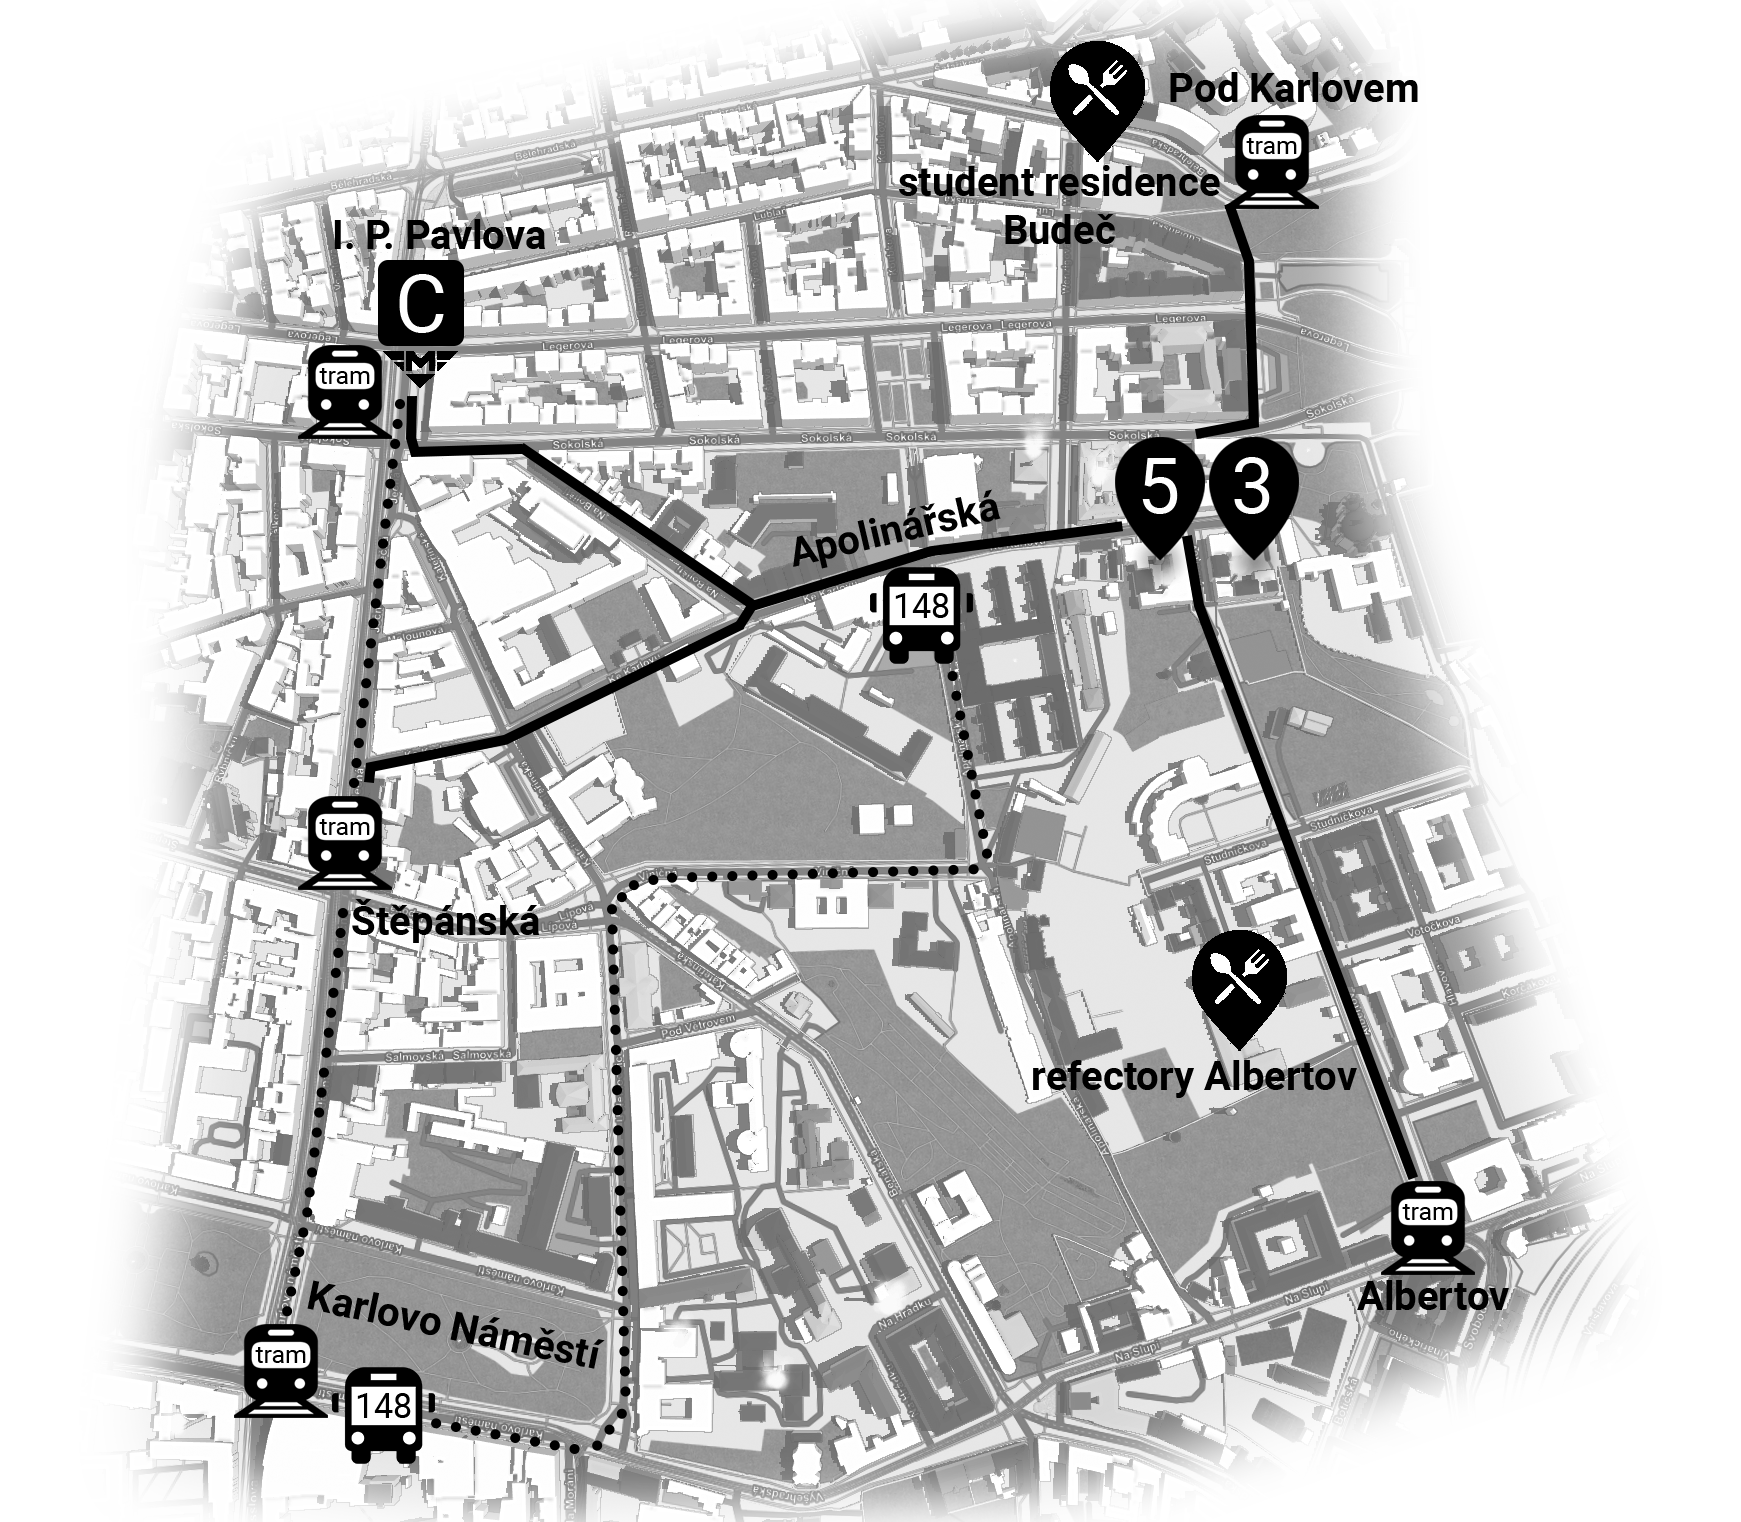
\includegraphics[width=\textwidth]{Images/mapaKarlov.png}\end{center}

\subsubsection*{Troja}
\begin{center}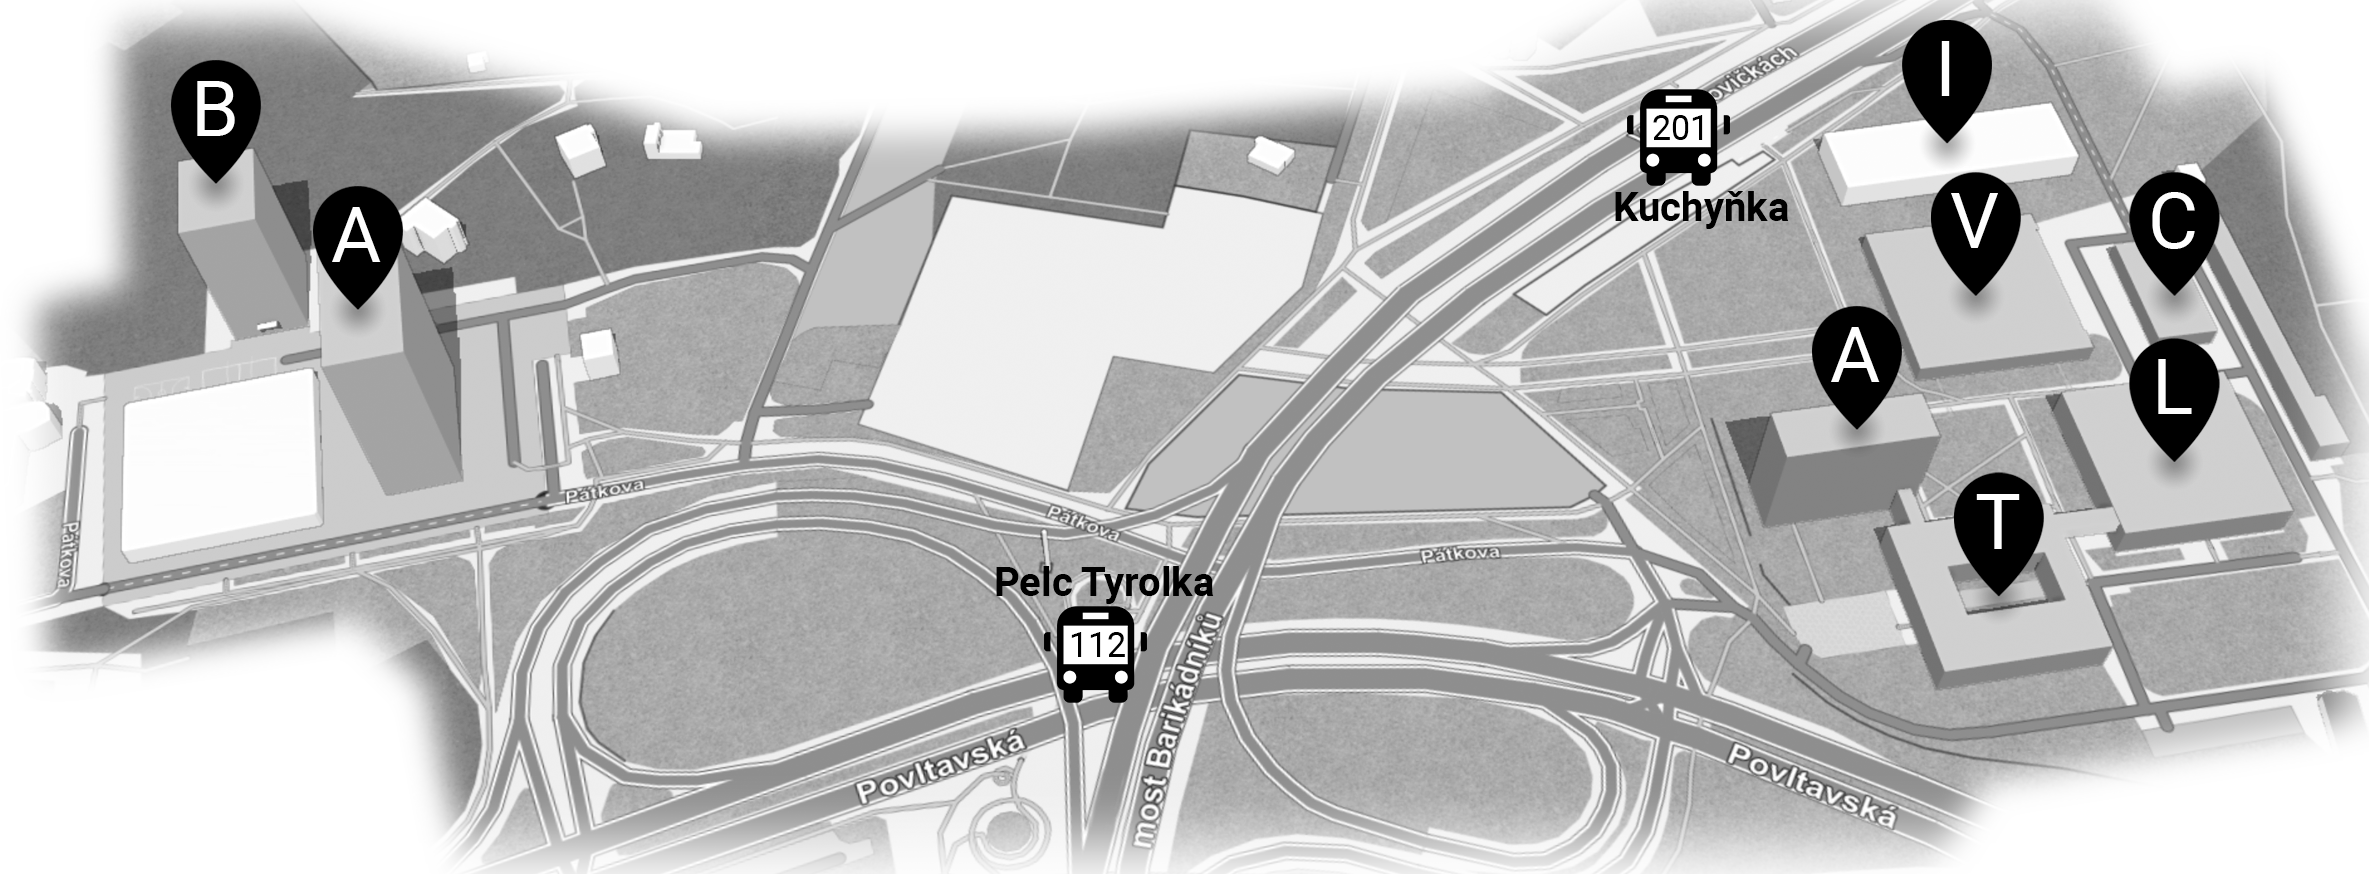
\includegraphics[width=\textwidth]{Images/mapaTroja.png}\end{center}

\subsubsection*{SCUK Hostivař}
\begin{center}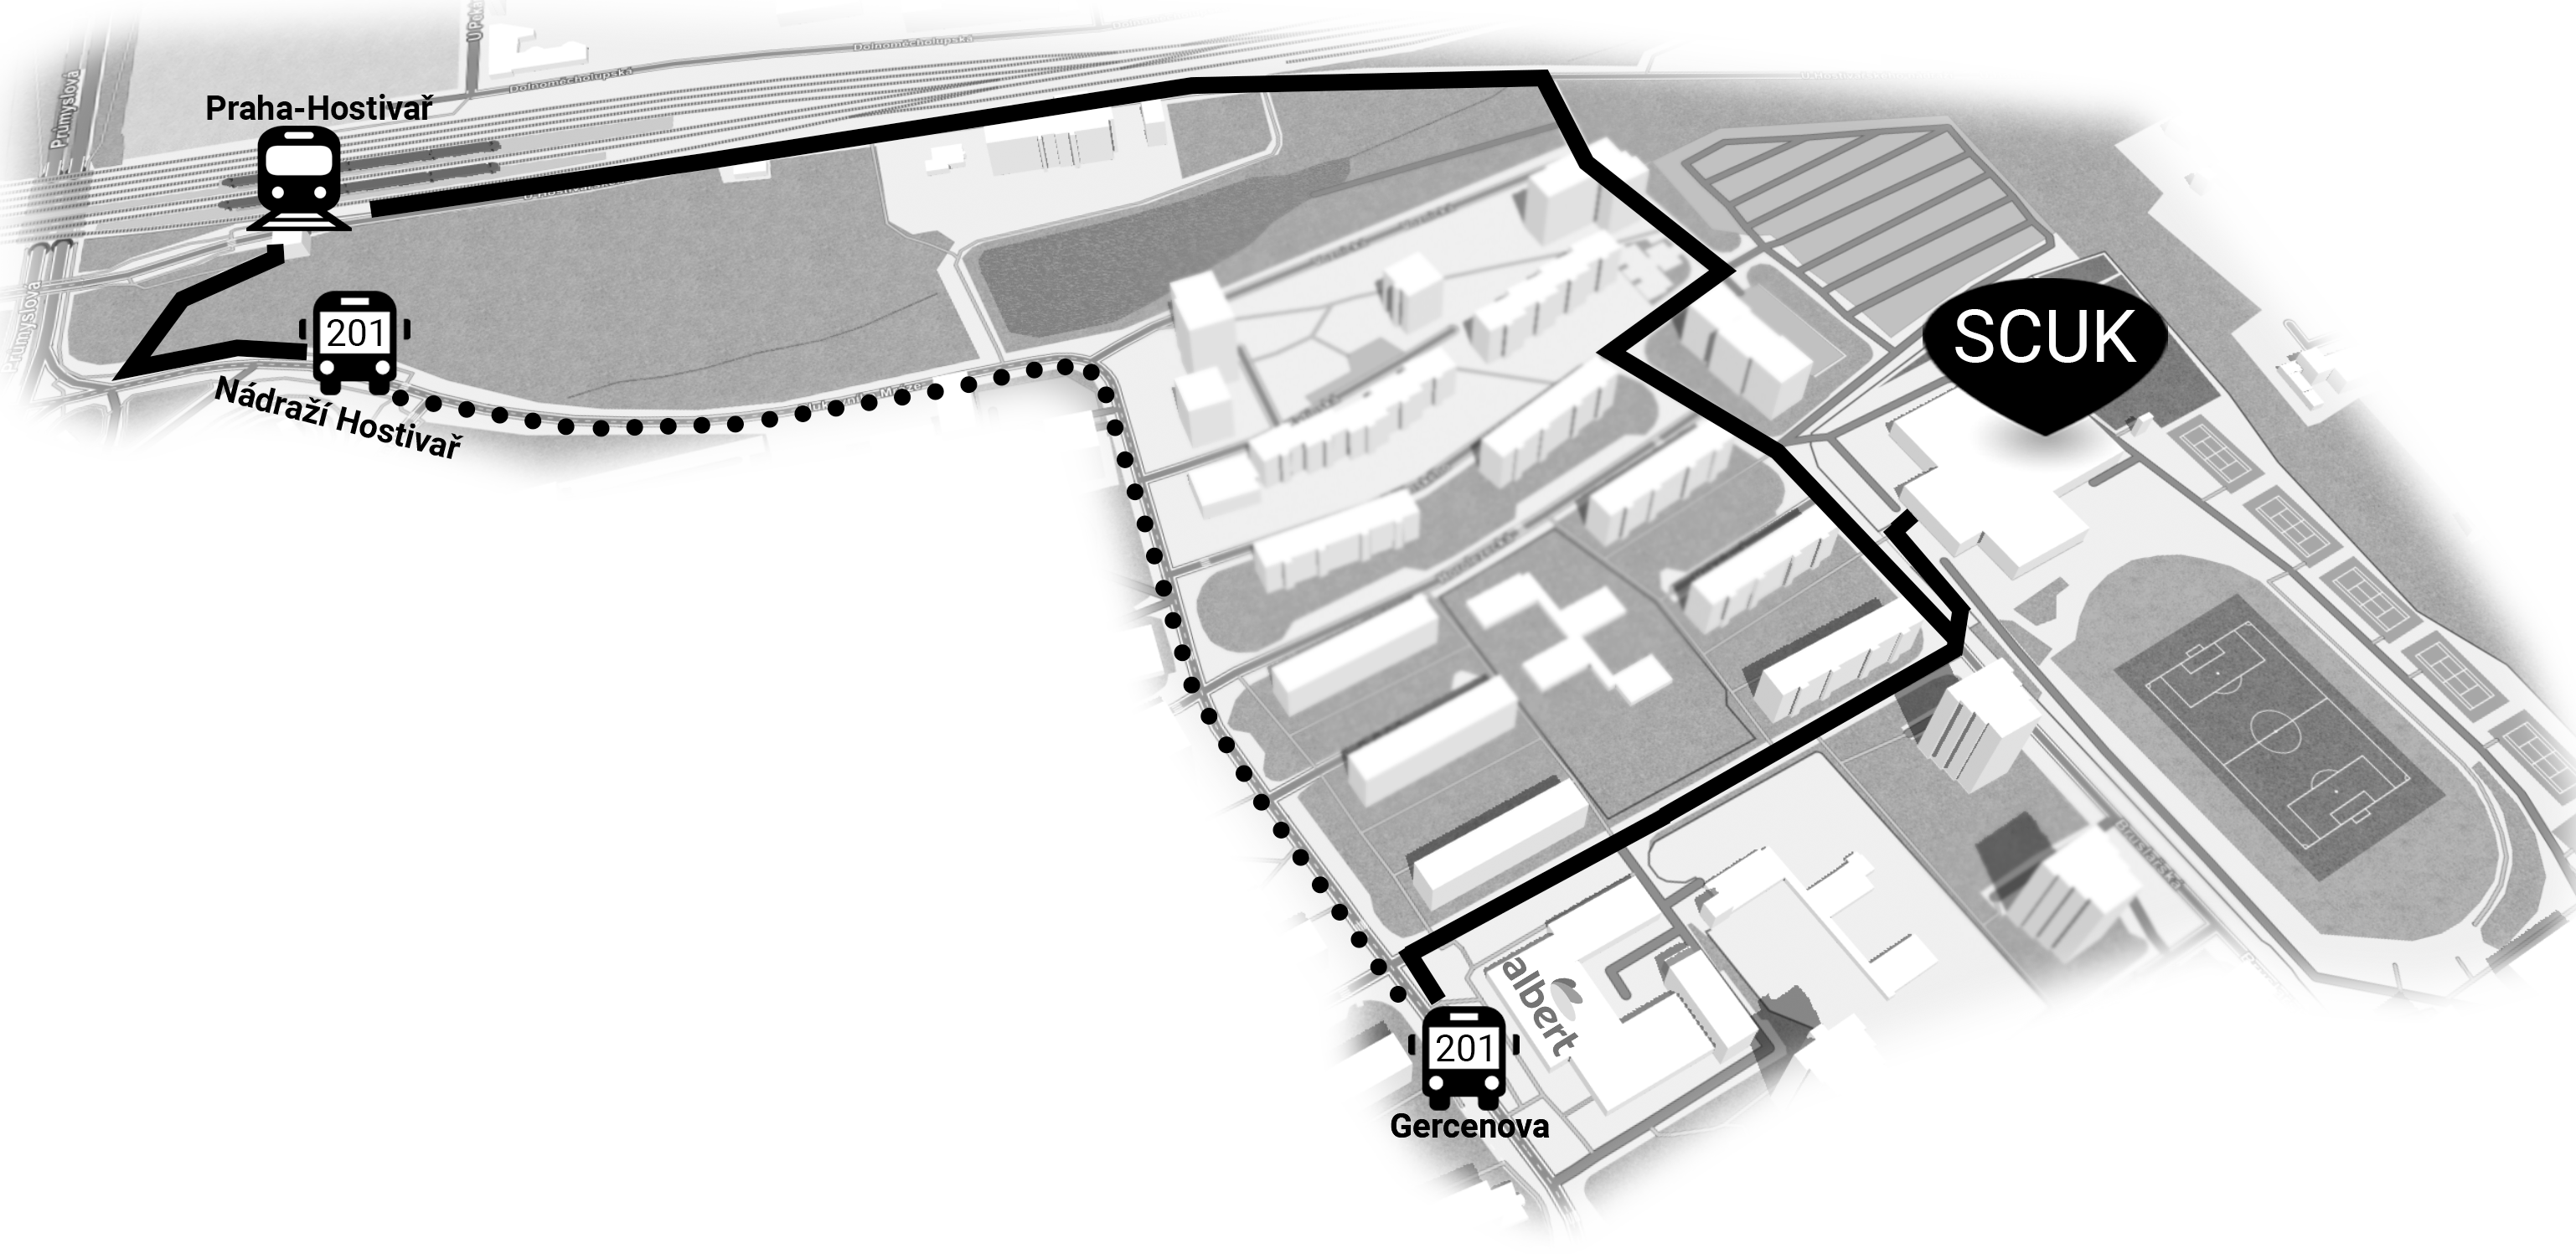
\includegraphics[width=\textwidth]{Images/mapaHostivar.png}\end{center}

\section{Conclusion}
So that is it. We believe that you liked our Cookbook and that you found it
useful. If there is any information you could not find here and thinks that it
should be included (or if you think that some of the information is of no use
whatsoever), reach as at \url{spolek@matfyzak.cz}.

\medskip

We wish you a pleasant stay in Prague.

\hskip 8cm \it Spolek Matfyzák
\if\readyForPrint0
	\newpage
\pagenumbering{gobble}
\section*{Useful links}
Are you holding a smartphone? Check out some useful links right now!

\vspace{20mm}

\begin{tabular}{cc}
    
\includegraphics[width=4cm]{Images/QR/is.png}&
    
\includegraphics[width=4cm]{Images/QR/studijni.png} \\
    Study Information System UK &
    Student Affairs Department MFF UK \\
    
    
\includegraphics[width=4cm]{Images/QR/skas.png}&
    
\includegraphics[width=4cm]{Images/QR/matfyzak.png} \\
    Student Chamber of the Academic\\Senate MFF UK (only in Czech) &
    Spolek Matfyzák (only in Czech) \\

    
\includegraphics[width=4cm]{Images/QR/facebook.png}&
    
\includegraphics[width=4cm]{Images/QR/knihovna.png} \\
    Facebook group for first year students &
    Library MFF UK (only in Czech)
\end{tabular}
\fi
\end{document}